% Options for packages loaded elsewhere
% Options for packages loaded elsewhere
\PassOptionsToPackage{unicode}{hyperref}
\PassOptionsToPackage{hyphens}{url}
\PassOptionsToPackage{dvipsnames,svgnames,x11names}{xcolor}
%
\documentclass[
  a4paper,
]{article}
\usepackage{xcolor}
\usepackage{amsmath,amssymb}
\setcounter{secnumdepth}{5}
\usepackage{iftex}
\ifPDFTeX
  \usepackage[T1]{fontenc}
  \usepackage[utf8]{inputenc}
  \usepackage{textcomp} % provide euro and other symbols
\else % if luatex or xetex
  \usepackage{unicode-math} % this also loads fontspec
  \defaultfontfeatures{Scale=MatchLowercase}
  \defaultfontfeatures[\rmfamily]{Ligatures=TeX,Scale=1}
\fi
\usepackage{lmodern}
\ifPDFTeX\else
  % xetex/luatex font selection
  \setmainfont[]{Latin Modern Roman}
  \setsansfont[]{Latin Modern Sans}
  \setmonofont[]{Latin Modern Mono}
\fi
% Use upquote if available, for straight quotes in verbatim environments
\IfFileExists{upquote.sty}{\usepackage{upquote}}{}
\IfFileExists{microtype.sty}{% use microtype if available
  \usepackage[]{microtype}
  \UseMicrotypeSet[protrusion]{basicmath} % disable protrusion for tt fonts
}{}
\makeatletter
\@ifundefined{KOMAClassName}{% if non-KOMA class
  \IfFileExists{parskip.sty}{%
    \usepackage{parskip}
  }{% else
    \setlength{\parindent}{0pt}
    \setlength{\parskip}{6pt plus 2pt minus 1pt}}
}{% if KOMA class
  \KOMAoptions{parskip=half}}
\makeatother
% Make \paragraph and \subparagraph free-standing
\makeatletter
\ifx\paragraph\undefined\else
  \let\oldparagraph\paragraph
  \renewcommand{\paragraph}{
    \@ifstar
      \xxxParagraphStar
      \xxxParagraphNoStar
  }
  \newcommand{\xxxParagraphStar}[1]{\oldparagraph*{#1}\mbox{}}
  \newcommand{\xxxParagraphNoStar}[1]{\oldparagraph{#1}\mbox{}}
\fi
\ifx\subparagraph\undefined\else
  \let\oldsubparagraph\subparagraph
  \renewcommand{\subparagraph}{
    \@ifstar
      \xxxSubParagraphStar
      \xxxSubParagraphNoStar
  }
  \newcommand{\xxxSubParagraphStar}[1]{\oldsubparagraph*{#1}\mbox{}}
  \newcommand{\xxxSubParagraphNoStar}[1]{\oldsubparagraph{#1}\mbox{}}
\fi
\makeatother


\usepackage{longtable,booktabs,array}
\usepackage{calc} % for calculating minipage widths
% Correct order of tables after \paragraph or \subparagraph
\usepackage{etoolbox}
\makeatletter
\patchcmd\longtable{\par}{\if@noskipsec\mbox{}\fi\par}{}{}
\makeatother
% Allow footnotes in longtable head/foot
\IfFileExists{footnotehyper.sty}{\usepackage{footnotehyper}}{\usepackage{footnote}}
\makesavenoteenv{longtable}
\usepackage{graphicx}
\makeatletter
\newsavebox\pandoc@box
\newcommand*\pandocbounded[1]{% scales image to fit in text height/width
  \sbox\pandoc@box{#1}%
  \Gscale@div\@tempa{\textheight}{\dimexpr\ht\pandoc@box+\dp\pandoc@box\relax}%
  \Gscale@div\@tempb{\linewidth}{\wd\pandoc@box}%
  \ifdim\@tempb\p@<\@tempa\p@\let\@tempa\@tempb\fi% select the smaller of both
  \ifdim\@tempa\p@<\p@\scalebox{\@tempa}{\usebox\pandoc@box}%
  \else\usebox{\pandoc@box}%
  \fi%
}
% Set default figure placement to htbp
\def\fps@figure{htbp}
\makeatother


% definitions for citeproc citations
\NewDocumentCommand\citeproctext{}{}
\NewDocumentCommand\citeproc{mm}{%
  \begingroup\def\citeproctext{#2}\cite{#1}\endgroup}
\makeatletter
 % allow citations to break across lines
 \let\@cite@ofmt\@firstofone
 % avoid brackets around text for \cite:
 \def\@biblabel#1{}
 \def\@cite#1#2{{#1\if@tempswa , #2\fi}}
\makeatother
\newlength{\cslhangindent}
\setlength{\cslhangindent}{1.5em}
\newlength{\csllabelwidth}
\setlength{\csllabelwidth}{3em}
\newenvironment{CSLReferences}[2] % #1 hanging-indent, #2 entry-spacing
 {\begin{list}{}{%
  \setlength{\itemindent}{0pt}
  \setlength{\leftmargin}{0pt}
  \setlength{\parsep}{0pt}
  % turn on hanging indent if param 1 is 1
  \ifodd #1
   \setlength{\leftmargin}{\cslhangindent}
   \setlength{\itemindent}{-1\cslhangindent}
  \fi
  % set entry spacing
  \setlength{\itemsep}{#2\baselineskip}}}
 {\end{list}}
\usepackage{calc}
\newcommand{\CSLBlock}[1]{\hfill\break\parbox[t]{\linewidth}{\strut\ignorespaces#1\strut}}
\newcommand{\CSLLeftMargin}[1]{\parbox[t]{\csllabelwidth}{\strut#1\strut}}
\newcommand{\CSLRightInline}[1]{\parbox[t]{\linewidth - \csllabelwidth}{\strut#1\strut}}
\newcommand{\CSLIndent}[1]{\hspace{\cslhangindent}#1}



\setlength{\emergencystretch}{3em} % prevent overfull lines

\providecommand{\tightlist}{%
  \setlength{\itemsep}{0pt}\setlength{\parskip}{0pt}}



 


\usepackage{booktabs}
\usepackage{longtable}
\usepackage{array}
\usepackage{multirow}
\usepackage{wrapfig}
\usepackage{float}
\usepackage{colortbl}
\usepackage{pdflscape}
\usepackage{tabu}
\usepackage{threeparttable}
\usepackage{threeparttablex}
\usepackage[normalem]{ulem}
\usepackage{makecell}
\usepackage{xcolor}
\usepackage{graphicx}
\usepackage{pdfpages}
\usepackage[a4paper, top=3cm, bottom=3cm, left=3.5cm, right=3.5cm]{geometry}
\usepackage{fancyhdr}

% --- Custom Title Page Definition (Robust Version) ---
\makeatletter
\renewcommand{\maketitle}{%
  \begin{titlepage}
    \thispagestyle{empty}
    \centering
    
    \vspace*{1cm}
    \includegraphics[width=6cm]{images/eth_logo.png}
    
    \vspace{2cm}
    {\Large Eidgenössische Technische Hochschule Zürich \par}
    {\Large Swiss Federal Institute of Technology Zurich \par}
    
    \vspace{2.5cm}
    {\Large Master's thesis\par}
    \vspace{0.5cm}
    {\large Master's degree programme in Agricultural Sciences\par}
    
    \vfill
    {\huge \bfseries \@title \par}
    
    \vfill
    {\Large \@author \par}
    {\large Student No. 13-938-311 \par}
    
    \vspace{2cm}
    \begin{tabular}{ll}
      \bfseries Supervisor: & Prof. Dr. Emmanuel Frossard \\
      & Institute of Agricultural Sciences, ETH Zurich \\
      \\
      \bfseries Advisor: & Dr. Frank Liebisch \\
      & Water Protection and Substance Flows, Agroscope Reckenholz \\
    \end{tabular}
    
    \vfill
    {\large \@date \par}
  \end{titlepage}
}
\makeatother
% --- End of Custom Title Page Definition ---

% --- Header Style Definition for Main Document ---
\fancypagestyle{fancy}{
  \fancyhf{}
  \fancyhead[L]{\nouppercase{\leftmark}}
  \fancyhead[R]{\thepage}
  \renewcommand{\headrulewidth}{0.4pt}
}
\makeatletter
\@ifpackageloaded{caption}{}{\usepackage{caption}}
\AtBeginDocument{%
\ifdefined\contentsname
  \renewcommand*\contentsname{Table of contents}
\else
  \newcommand\contentsname{Table of contents}
\fi
\ifdefined\listfigurename
  \renewcommand*\listfigurename{List of Figures}
\else
  \newcommand\listfigurename{List of Figures}
\fi
\ifdefined\listtablename
  \renewcommand*\listtablename{List of Tables}
\else
  \newcommand\listtablename{List of Tables}
\fi
\ifdefined\figurename
  \renewcommand*\figurename{Figure}
\else
  \newcommand\figurename{Figure}
\fi
\ifdefined\tablename
  \renewcommand*\tablename{Table}
\else
  \newcommand\tablename{Table}
\fi
}
\@ifpackageloaded{float}{}{\usepackage{float}}
\floatstyle{ruled}
\@ifundefined{c@chapter}{\newfloat{codelisting}{h}{lop}}{\newfloat{codelisting}{h}{lop}[chapter]}
\floatname{codelisting}{Listing}
\newcommand*\listoflistings{\listof{codelisting}{List of Listings}}
\makeatother
\makeatletter
\makeatother
\makeatletter
\@ifpackageloaded{caption}{}{\usepackage{caption}}
\@ifpackageloaded{subcaption}{}{\usepackage{subcaption}}
\makeatother
\usepackage{bookmark}
\IfFileExists{xurl.sty}{\usepackage{xurl}}{} % add URL line breaks if available
\urlstyle{same}
\hypersetup{
  pdftitle={P-release kinetic as a predictor for P-availability in Swiss cropping systems},
  colorlinks=true,
  linkcolor={blue},
  filecolor={Maroon},
  citecolor={Blue},
  urlcolor={Blue},
  pdfcreator={LaTeX via pandoc}}


\title{P-release kinetic as a predictor for P-availability in Swiss
cropping systems}
\author{Marc Jerónimo Pérez y Ropero}
\date{2025-09-12}
\begin{document}
\maketitle
\begin{abstract}
Traditional static soil tests (STPs) for phosphorus (P) often fail to
predict agronomic outcomes because they do not account for the kinetic
nature of P supply to plant roots. This thesis investigated whether P
desorption kinetic parameters could serve as more effective predictors.
Using soils from the long-term Swiss agricultural experiment (STYCS), a
sequential extraction method was refined and modeled with a non-linear
approach to derive the desorbable P pool (\(P_{desorb}\)) and a rate
constant (\emph{k}). The predictive power of these kinetic parameters
was compared against standard Swiss STPs (\(P_{CO_2}\) and
\(P_{AAE10}\)) for various agronomic outcomes using linear mixed-effects
models. The results revealed a highly context-dependent performance. For
predicting site-normalized yield, STPs were superior, while for
national-normalized yield and P-uptake, both methods performed poorly,
with their predictive signals being overshadowed by dominant
pedoclimatic factors. Furthermore, the two STP methods provided largely
redundant information, as their combination did not improve predictive
power. The most significant finding was the exceptional success of the
kinetic model in predicting the long-term P-Balance, a key indicator of
nutrient stewardship. The \(P_{desorb}\) parameter alone explained 57\%
of the variance, whereas STP models showed no predictive power. This
study concludes that the ideal soil P test is purpose-dependent: while
traditional STPs remain adequate for within-field fertility management,
kinetic parameters are a vastly superior tool for assessing the
long-term P status and sustainability of agricultural soils.
\end{abstract}

\cleardoublepage
\tableofcontents
\cleardoublepage 
\pagestyle{fancy}
\pagenumbering{arabic}


\section{Introduction}\label{introduction}

\subsection{The Complexity of
Phosphorus}\label{the-complexity-of-phosphorus}

Phosphorus (P) is an essential macronutrient for all known life, forming
a critical part of DNA and energy-transfer molecules (Berg et al., 2019;
National Institutes of Health, Office of Dietary Supplements, 2023;
Nelson et al., 2021). In soils---where organic, mineral, and aqueous
phases interface---its behavior is complex. In the presence of oxygen, P
exists almost exclusively as orthophosphate (\(PO_4^{3-}\)) and its
protonated forms (\(HPO_4^{2-}\) or \(H_2PO_4^{-}\)), depending on the
soil pH (Brady \& Weil, 2016; Sparks, 2003). These dissolved phosphate
species are highly reactive; they are subject to adsorption onto the
surfaces of clays and oxides and can precipitate with cations like
calcium, iron, and aluminum to form minerals with low solubility (Bohn
et al., 2002; Hinsinger, 2001; Sposito, 2008). Consequently, while total
soil P concentrations can be substantial, often ranging from 200 to 3000
mg kg⁻¹, the concentration of orthophosphate in the soil solution---the
form directly acquired by plant roots---is typically minuscule, often in
the range of 0.001 to 1 mg L⁻¹. This vast difference between the total
phosphorus stock and the infinitesimally small plant-available pool
represents a central challenge for global agricultural productivity
(Brady \& Weil, 2016; Holford, 1997; Sposito, 2008). This creates a
profound agronomic and environmental dilemma: while the majority of
applied P fertilizer is rapidly immobilized in the soil and remains
unavailable to crops, the fraction that is lost from fields via runoff
and erosion becomes a potent environmental pollutant. This fugitive P is
a primary driver of eutrophication in freshwater ecosystems, which are
often naturally P-limited Sharpley et al. (2003).

\textbf{Soil organic matter (SOM) adds another layer of complexity to
these interactions.} Organic acids released during the decomposition of
SOM can compete with phosphate for the same adsorption sites on mineral
surfaces, which can increase P concentrations in the soil solution.
Furthermore, humic substances can form stable complexes with cations
like Al³⁺ and Fe³⁺, preventing them from precipitating phosphate and
thereby enhancing its availability (Gerke, 2010; Stevenson, 1994).

\subsection{From Static Measurements to Dynamic
Understanding}\label{from-static-measurements-to-dynamic-understanding}

To manage this challenge, soil testing methods were developed to
estimate plant-available phosphorus. These tests are designed to measure
two key components of P availability: the \textbf{intensity factor},
which is the concentration of P in the soil solution at a given moment,
and the \textbf{capacity factor}, which represents the pool of weakly
adsorbed P that can readily replenish the soil solution (Frossard et
al., 2000). Traditional methods used in Switzerland and the surrounding
DACH region, which are standardized by organizations like the
\textbf{VDLUFA} (Verband Deutscher Landwirtschaftlicher Untersuchungs-
und Forschungsanstalten) and form the basis of Swiss fertilization
guidelines (\textbf{GRUD}; Grundlagen für die Düngung), often employ a
dual-method approach. This strategy is designed to assess both the
P-intensity and P-capacity factors separately by using a combination of
weak and strong extractants. Weak extractants, such as CO₂-saturated
water, are intended to measure the readily available P in the soil
solution (intensity). In contrast, stronger, often chelate-based
extractants like ammonium acetate EDTA (AAE10) or
calcium-acetate-lactate (CAL) are used to estimate the more tightly
bound, resupply pool of phosphorus (capacity) (Forschungsanstalt für
Agrarökologie und Landbau (FAL), 1996; Verband Deutscher
Landwirtschaftlicher Untersuchungs- und Forschungsanstalten (VDLUFA),
2000). While this dual approach is logical, other international
standards, such as the widely used Olsen-P method, rely on a single
extraction to provide an index of plant-available P (Olsen et al.,
1954). Although these static tests are invaluable for basic fertility
assessment, they do not capture the dynamic nature of P supply. A
crucial missing piece of information is the rate at which P is
replenished into the soil solution from the solid phase after being
taken up by plant roots. This replenishment rate, or \textbf{``kinetic
factor''}, is vital for sustaining crop growth, especially during
periods of high demand Frossard et al. (2000).

The importance of these dynamics is not a new concept. As early as 1982,
\textbf{Flossmann and Richter} argued that characterizing the kinetics
of P release was essential for refining fertilizer recommendations
beyond what static tests alone could offer (Flossmann \& Richter, 1982).
Modern research has reinforced this view, showing that fertilization
strategies based solely on maintaining a critical soil test P (STP)
concentration can be inefficient (McDowell \& Sharpley, 2001; Rowe et
al., 2016). In Switzerland, this has led to the accumulation of ``legacy
P'' in many agricultural soils. Additionally, understanding the release
kinetics of this legacy P is key to both improving nutrient use
efficiency and protecting water ecosystems and reserves (Hirte et al.,
2018). Furthermore, critical STP levels are not constant; they are
influenced by pedoclimatic factors like soil texture and temperature,
making a ``one-size-fits-all'' approach to fertilization suboptimal
(Bell et al., 2013; Hirte, Richner, et al., 2021; Sims \& Sharpley,
2005).

\subsection{Objectives and Research
Questions}\label{objectives-and-research-questions}

An ideal set of parameters for phosphorus (P) management must move
beyond simple agronomic sufficiency to encompass both environmental
stewardship and the biophysical realities of nutrient acquisition by
plants. To be truly effective, such parameters must: (1) be sensitive to
changes in the soil P status resulting from fertilizer inputs and crop
removal (the P balance) (Frossard et al., 2000; Johnston et al., 2001);
(2) correlate with the risk of P loss to the environment (P export)
(Sharpley et al., 2000); and (3), most critically, reflect the kinetic
nature of P supply to plant roots, which is governed by the slow
diffusion of phosphate in the soil solution (Kuang et al., 2012; Nye \&
Tinker, 2000).

This thesis hypothesizes that kinetic parameters describing P
desorption, derived from a simple laboratory extraction, can serve as
effective predictors for agronomic outcomes. To test this, soils were
sourced from the long-term Swiss agricultural experiment STYCS (Hirte,
Stüssel, et al., 2021). The experiment's multi-decade history has
established stable P equilibria across a wide and deliberately created
gradient of P availability (from 0\% to 167\% of recommended
fertilization), allowing for robust modeling of crop responses.
Furthermore, the trial encompasses six sites with diverse pedoclimatic
conditions, ensuring that any findings have broad applicability across
different Swiss agricultural landscapes. This study employs a modified
version of the Flossmann \& Richter kinetic test to derive the
desorption rate (k) and the desorbable P pool (\(P_{desorb}\)). The
performance of these new kinetic parameters will be compared against
standard STP methods (\(P_{CO_2}\) and \(P_{AAE10}\)) by addressing the
following research questions:

\subsubsection{Research Questions and
Hypotheses}\label{research-questions-and-hypotheses}

Research Question 1: How well do standard soil test P (STP) methods
predict agronomic outcomes and how do they relate to fundamental soil
properties?

\begin{itemize}
\item
  \textbf{Hypothesis 1a (Agronomic Performance):} The standard STP
  methods (\(P_{CO_2}\) and \(P_{AAE10}\)), which measure the P
  \emph{capacity} (the size of the readily available pool), will show a
  significant correlation with the P-Balance, as this is directly
  influenced by P inputs (Johnston et al., 2001). However, they will be
  weak predictors of relative crop yield and P-uptake, as these
  agronomic outcomes are more dependent on the \emph{rate} of P supply
  throughout the growing season (Hirte, Stüssel, et al., 2021).
\item
  \textbf{Hypothesis 1b (Relation to Soil Properties):} The measured STP
  values will be positively correlated with soil clay and organic carbon
  content, reflecting the greater number of sorption sites in these
  soils (Brady \& Weil, 2016). Conversely, the P\_AAE10 measurement will
  be negatively correlated with soil pH, particularly in soils with a
  \(pH > 6.8\), due to the chelation of \(Ca^{2+}\) and \(Mg^{2+}\) by
  the EDTA in the extractant, which reduces its effectiveness
  (Forschungsanstalt für Agrarökologie und Landbau (FAL), 1996).
\end{itemize}

Research Question 2: Can P desorption kinetics be reliably characterized
for the diverse soils of the STYCS trial, and how do the derived kinetic
parameters relate to soil properties?

\begin{itemize}
\item
  \textbf{Hypothesis 2a (Methodological Feasibility):} The P desorption
  process in the STYCS soils will follow a first-order kinetic model.
  However, the original linear estimation method proposed by Flossmann
  \& Richter (1982) may be inaccurate because it relies on a potentially
  overestimated desorbable P pool (\(P_{desorb}\)). A non-linear
  modeling approach will provide more robust and replicable estimates of
  both the desorption rate constant (\emph{k}) and the desorbable P pool
  (\(P_{desorb}\)) (Kuang et al., 2012).
\item
  \textbf{Hypothesis 2b (Relation to Soil Properties):} The kinetic
  parameters will be significantly influenced by soil composition. The
  desorbable P pool (\(P_{desorb}\)) is expected to correlate positively
  with clay and organic matter content, which provide sorption surfaces.
  The rate constant (\emph{k}) is expected to be influenced by pH, as
  the speciation of orthophosphate changes, affecting its interaction
  with mineral surfaces and its mobility (Sparks, 2003).
\end{itemize}

Research Question 3: Can kinetic parameters significantly improve the
prediction of agronomic outcomes compared to standard static STP
methods?

\begin{itemize}
\tightlist
\item
  \textbf{Hypothesis 3 (Improved Predictive Power):} Because plant P
  uptake is fundamentally limited by the slow diffusion of phosphate to
  the root surface, a dynamic measure is required for accurate
  prediction (Nye \& Tinker, 2000). Therefore, a model incorporating the
  kinetic parameters (\emph{k} and \(P_{desorb}\)), which together
  describe the replenishment rate of the soil solution, will explain a
  significantly greater proportion of the variance in relative yield and
  P-uptake compared to models based solely on the static STP
  measurements (Fardeau et al., 1991; Frossard et al., 2000).
\end{itemize}

\newpage

\section{Materials and Methods}\label{sec-materials-and-methods}

\subsection{The Long-Term Phosphorus Fertilization
Experiment}\label{sec-the-long-term-phosphorus-fertilization-experiment}

The soil samples for this thesis originate from a set of six long-term
field trials in Switzerland, established by Agroscope between 1989 and
1992. The primary objective of these experiments was to validate and
re-evaluate Swiss phosphorus (P) fertilization guidelines by assessing
long-term crop yield responses to varying P inputs across different
pedoclimatic conditions. A detailed description of the experimental
design and site characteristics can be found in Hirte, Richner, et al.
(2021).

The experiment was set up as a \textbf{completely randomized block
design} with four field replications at each site. The core of the
experiment consists of six fixed-plot treatments representing different
P fertilization levels, which were applied annually as superphosphate
before tillage and sowing. These levels were based on percentages of the
officially recommended P inputs: 0\% (Zero), 33\% (Deficit), 67\%
(Reduced), 100\% (Norm), 133\% (Elevated), and 167\% (Surplus).

\subsection{Experimental Sites}\label{sec-experimental-sites}

The six experimental sites are located in the main crop-growing regions
of Switzerland: \textbf{Rümlang-Altwi (ALT)}, \textbf{Cadenazzo (CAD)},
\textbf{Ellighausen (ELL)}, \textbf{Grabs (GRA)}, \textbf{Oensingen
(OEN)}, and \textbf{Zurich-Reckenholz (REC)}. The key soil properties
are summarized below.

\begin{longtable}[]{@{}
  >{\raggedright\arraybackslash}p{(\linewidth - 10\tabcolsep) * \real{0.0704}}
  >{\raggedright\arraybackslash}p{(\linewidth - 10\tabcolsep) * \real{0.3099}}
  >{\raggedleft\arraybackslash}p{(\linewidth - 10\tabcolsep) * \real{0.1268}}
  >{\raggedleft\arraybackslash}p{(\linewidth - 10\tabcolsep) * \real{0.1268}}
  >{\raggedleft\arraybackslash}p{(\linewidth - 10\tabcolsep) * \real{0.2394}}
  >{\raggedleft\arraybackslash}p{(\linewidth - 10\tabcolsep) * \real{0.1268}}@{}}

\caption{\label{tbl-sites-corrected}Soil characteristics of the six
long-term experimental sites. Data adapted from Hirte et al.~(2021).}

\tabularnewline

\toprule\noalign{}
\begin{minipage}[b]{\linewidth}\raggedright
Site
\end{minipage} & \begin{minipage}[b]{\linewidth}\raggedright
Soil Type (WRB)
\end{minipage} & \begin{minipage}[b]{\linewidth}\raggedleft
Clay (\%)
\end{minipage} & \begin{minipage}[b]{\linewidth}\raggedleft
Sand (\%)
\end{minipage} & \begin{minipage}[b]{\linewidth}\raggedleft
Organic C (g/kg)
\end{minipage} & \begin{minipage}[b]{\linewidth}\raggedleft
pH (H2O)
\end{minipage} \\
\midrule\noalign{}
\endhead
\bottomrule\noalign{}
\endlastfoot
ALT & Calcaric Cambisol & 22 & 48 & 21 & 7.9 \\
CAD & Eutric Fluvisol & 8 & 40 & 14 & 6.3 \\
ELL & Eutric Cambisol & 33 & 31 & 23 & 6.6 \\
GRA & Calcaric Fluvisol & 17 & 34 & 16 & 8.3 \\
OEN & Gleyic-calc. Cambisol & 37 & 32 & 24 & 7.1 \\
REC & Eutric Gleysol & 39 & 25 & 27 & 7.4 \\

\end{longtable}

Soil samples for this thesis were collected in the year 2022 from the
topsoil layer (0-20 cm).

\subsection{Phosphorus Desorption
Kinetics}\label{sec-phosphorus-desorption-kinetics}

The analysis of phosphorus (P) desorption kinetics was based on the
principles of sequential extraction established by Flossmann \& Richter
(1982). The original method is described below, followed by the specific
protocol adapted for this study.

\subsubsection{Original Method of Flossmann and
Richter}\label{original-method-of-flossmann-and-richter}

The foundational method aims to characterize the P replenishment
capacity of the soil. The procedure is as follows:

\begin{enumerate}
\def\labelenumi{\arabic{enumi}.}
\tightlist
\item
  \textbf{Removal of Soluble P}: 17.5 g of air-dried soil is shaken with
  350 ml of deionized water for one hour at 120 Hz in a horizontal
  soil-shaker. The suspension is centrifuged at 4000 rpm for 15 minutes
  and the supernatant is decanted to remove the readily soluble P
  fraction.
\item
  \textbf{Kinetic Extraction}: The remaining soil pellet is resuspended
  with another 350 ml of deionized water. Subsamples of the suspension
  are taken at specific time intervals (e.g., 10, 30, and 120 minutes).
\item
  \textbf{Analysis}: The P concentration in the subsamples is determined
  colorimetrically.
\end{enumerate}

\subsubsection{Adapted Kinetic Protocol for This
Study}\label{sec-adapted-kinetic-protocol-for-this-study}

For this thesis, the original method was modified to capture the
desorption process with a higher temporal resolution.

\begin{enumerate}
\def\labelenumi{\arabic{enumi}.}
\item
  \textbf{Pre-washing to Remove Soluble P}: A pre-washing step was
  performed to remove the readily soluble P fraction. 10 g of air-dried
  soil was suspended in 200 ml of deionized water and shaken for 60
  minutes at 120 Hz. The suspension was then centrifuged for 15 minutes
  at 4000 rpm, and the supernatant containing the soluble P was
  discarded.
\item
  \textbf{Kinetic Extraction}: The remaining soil pellet was resuspended
  in 200 ml of fresh deionized water. The suspension was shaken
  continuously, and subsamples were taken at eight time points to
  generate a detailed kinetic curve: \textbf{2, 4, 10, 15, 20, 30, 45,
  and 60 minutes}.
\item
  \textbf{Analysis}: Each subsample was immediately filtered. The
  concentration of orthophosphate in the filtered extracts was
  determined colorimetrically using the \textbf{malachite green method}
  (Van Veldhoven \& Mannaerts, 1987).
\end{enumerate}

\subsection{Statistical Analysis}\label{sec-statistical-analysis}

\subsubsection{Software and Statistical
Environment}\label{software-and-statistical-environment}

All data processing, statistical modeling, and visualization were
conducted using the R programming language (v. 4.2.2) (R Core Team,
2022). The primary packages used for the analysis were: - \texttt{nlme}
(Pinheiro et al., 2022) for fitting the non-linear mixed-effects models
to the kinetic data. - \texttt{lme4} (Bates et al., 2015) and
\texttt{lmerTest} (Kuznetsova et al., 2017) for fitting and testing the
linear mixed-effects models for agronomic and soil property analyses. -
\texttt{mlr3} (Lang et al., 2019) for the systematic feature selection
and model validation workflow.

\subsubsection{Modeling of Desorption
Kinetics}\label{sec-modeling-of-desorption-kinetics}

To derive the kinetic parameters, a non-linear mixed-effects model was
implemented using the \texttt{nlme} package. This approach was chosen to
simultaneously estimate the rate constant (\emph{k}) and the maximum
desorbable P (\(P_{desorb}\)) for each soil sample. The model was fitted
to the exact solution of the first-order rate equation:

\[P(t) = P_{desorb} \times (1 - e^{-k \times t'})\]

Where \(P(t)\) is the P concentration at time \(t\), and \(t'\) is an
adjusted time (\(t_{min}\) + 3 min) to account for the rapid initial
dissolution of P that occurs before the first measurement. In this
mixed-effects framework, the overall mean values for \(P_{desorb}\) and
\emph{k} were modeled as \textbf{fixed effects}, while sample-specific
deviations from these fixed effects were modeled as \textbf{random
effects} to capture the unique desorption characteristics of each
individual soil sample.

\subsubsection{Comparative Modeling of Soil and Agronomic
Parameters}\label{comparative-modeling-of-soil-and-agronomic-parameters}

To test the hypotheses of this thesis, two distinct sets of linear
mixed-effects models were constructed.


\begin{longtable}[]{@{}
  >{\raggedright\arraybackslash}p{(\linewidth - 6\tabcolsep) * \real{0.0807}}
  >{\raggedright\arraybackslash}p{(\linewidth - 6\tabcolsep) * \real{0.1615}}
  >{\raggedright\arraybackslash}p{(\linewidth - 6\tabcolsep) * \real{0.0932}}
  >{\raggedright\arraybackslash}p{(\linewidth - 6\tabcolsep) * \real{0.6646}}@{}}

\caption{\label{tbl-variables}Description of variables used in the
agronomic and soil models.}

\tabularnewline

\toprule\noalign{}
\begin{minipage}[b]{\linewidth}\raggedright
Abbreviation
\end{minipage} & \begin{minipage}[b]{\linewidth}\raggedright
Variable
\end{minipage} & \begin{minipage}[b]{\linewidth}\raggedright
Unit
\end{minipage} & \begin{minipage}[b]{\linewidth}\raggedright
Description
\end{minipage} \\
\midrule\noalign{}
\endhead
\bottomrule\noalign{}
\endlastfoot
\(Y_{rel}\) & Relative Yield & unitless & Plot yield normalized by the
national mean yield for that year and crop. \\
\(Y_{norm}\) & Normalized Yield & unitless & Plot yield normalized by
the site-specific median yield of the highest P treatment for that year
and crop. \\
\(P_{up}\) & P Uptake & kg P ha⁻¹ & Total P removed by the harvested
crop biomass over a growing season. \\
\(P_{bal}\) & P Balance & kg P ha⁻¹ & Net P budget, calculated as P
inputs (fertilizer) minus P outputs (uptake). \\
\(k\) & Rate Constant & min⁻¹ & First-order rate constant of P
desorption, representing the speed of P release. \\
\(P_{desorb}\) & Desorbable P & mg P L⁻¹ & Maximum desorbable P,
representing the size of the readily available P pool. \\
\(J_0\) & Initial P Flux & mg P L⁻¹ min⁻¹ & Product of \(k\) and
\(P_{desorb}\), representing the initial flux of P from the soil. \\
\(P_{CO2}\) & Water-Soluble P & mg P kg⁻¹ & Plant-available P measured
by CO₂-saturated water extraction
(Forschungsanstalt für Agrarökologie und Landbau (FAL), 1996). \\
\(P_{AAE10}\) & Chelate-Extractable P & mg P kg⁻¹ & Plant-available P
measured by the ammonium-acetate-EDTA extraction method
(Forschungsanstalt für Agrarökologie und Landbau (FAL), 1996). \\
\(Al_d\) & Dithionite-Extractable Al & mg Al kg⁻¹ & Free Al oxides
(crystalline and amorphous) extracted with
dithionite-citrate-bicarbonate
(Mehra \& Jackson, 1960). \\
\(Fe_d\) & Dithionite-Extractable Fe & mg Fe kg⁻¹ & Free Fe oxides
(crystalline and amorphous) extracted with
dithionite-citrate-bicarbonate
(Mehra \& Jackson, 1960). \\

\end{longtable}

\subsubsection{Model Assumptions and
Diagnostics}\label{model-assumptions-and-diagnostics}

The validity of the linear mixed-effects models (\texttt{lmer}) relies
on several key assumptions, primarily that the model residuals are
normally distributed and homoscedastic (i.e., have constant variance
across the range of predicted values). Prior to finalizing the models,
these assumptions were rigorously checked through visual inspection of
diagnostic plots, such as quantile-quantile (Q-Q) plots of the residuals
and plots of residuals versus fitted values.

Initial exploratory data analysis revealed that several of the predictor
variables, most notably the desorbable P pool (\(P_{desorb}\) or PS),
were strongly right-skewed. Using such variables directly in the linear
models would violate the assumptions of linearity and homoscedasticity,
leading to potentially biased and unreliable coefficient estimates.

To address this, various transformations (including square root and
logarithmic) were tested on the skewed variables. The natural
log-transformation (\texttt{log()}) was found to be the most effective
at normalizing the distribution of \(P_{desorb}\) and producing
well-behaved model residuals that more closely met the required
assumptions. Therefore, \texttt{log(PS)} was used as a fixed effect in
all subsequent agronomic models to ensure the statistical validity of
the results.

\paragraph{Models of P Availability Metrics as a Function of Soil
Properties}\label{models-of-p-availability-metrics-as-a-function-of-soil-properties}

First, to investigate the underlying soil-chemical drivers of the
different P availability metrics (both kinetic and static), a series of
models was built to predict each metric from key soil properties.

\begin{itemize}
\tightlist
\item
  \textbf{Fixed Effects Structure:} The fixed effects were identical for
  all models in this category and included the primary soil physical and
  chemical properties: clay content, silt content, pH, organic carbon
  content, and dithionite-extractable iron (\(Fe_d\)) and aluminum
  (\(Al_d\)).
\item
  \textbf{Random Effects Structure:} The random effects structure
  accounted for the nested design of the STYCS experiment, with random
  intercepts for \texttt{year}, \texttt{Site}, \texttt{Site:block}, and
  \texttt{Site:Treatment}.
\end{itemize}

\paragraph{Comparative Models of Agronomic
Outcomes}\label{comparative-models-of-agronomic-outcomes}

Second, the predictive power of the kinetic parameters was directly
compared against that of the standard STP methods (``GRUD'' system). For
each agronomic response variable (Normalized Yield, P Uptake, and P
Balance), two competing models were built. These models shared an
identical random effects structure to ensure a fair comparison,
differing only in their fixed effects.

\begin{itemize}
\item
  \textbf{Random Effects Structure (for all agronomic models):} The
  structure
  \texttt{(1\textbar{}year)\ +\ (1\textbar{}Site)\ +\ (1\textbar{}Site:block)}
  was used to control for variations due to the growing season,
  location, and in-field spatial differences.
\item
  \textbf{Model 1: The Kinetic Approach}

  \begin{itemize}
  \tightlist
  \item
    \textbf{Fixed Effects:} This model used the kinetic parameters and
    their interaction: \texttt{k\ *\ log(PS)}. The interaction term
    tests the hypothesis that the benefit of a large desorbable P pool
    (\texttt{PS}) depends on the \emph{rate} (\texttt{k}) at which it
    can be accessed.
  \end{itemize}
\item
  \textbf{Model 2: The Standard STP (GRUD) Approach}

  \begin{itemize}
  \tightlist
  \item
    \textbf{Fixed Effects:} This model used the two standard Swiss soil
    tests and their interaction: \texttt{P\_CO2\ *\ P\_AAE10}.
  \end{itemize}
\end{itemize}

The relative performance of these two sets of models was then evaluated
to determine whether the kinetic parameters provided a significant
improvement in predictive power for key agronomic outcomes. Further the
relative performance of these two approaches, along with other
combinations of predictor sets, was rigorously evaluated using a machine
learning benchmark workflow implemented in the \texttt{mlr3} package
(Lang et al., 2019). The predictive power of each predictor set was
quantified using \textbf{5-fold cross-validation}. Performance was
measured as the percentage of explained variance on the hold-out data (1
- MSE / Var(y)), providing a robust and unbiased estimate of how well
each model would generalize to new data. This benchmark allowed for a
direct comparison of the information content provided by the kinetic
parameters versus the standard soil tests for predicting key agronomic
outcomes.

\newpage

\section{Results}\label{results}

The results of this study are presented in two main parts. First, the
development and validation of the phosphorus (P) desorption kinetic
model are detailed, justifying the final modeling approach. Second, the
descriptive trends of both agronomic outcomes and soil P parameters in
response to long-term fertilization and site differences are explored
visually. Finally, the predictive power of the kinetic and standard P
parameters is formally evaluated using linear mixed-effects models.

\subsection{Establishment of the P-Desorption Kinetic
Model}\label{establishment-of-the-p-desorption-kinetic-model}

The primary goal was to derive two key parameters for each soil sample:
the desorbable P pool (\(P_{desorb}\)) and the rate constant (\(k\)).
The analysis proceeded in two stages: an initial test of a linearized
model, followed by the implementation of a more robust non-linear model.

\subsubsection{Initial Approach: Failure of the Linearized
Model}\label{initial-approach-failure-of-the-linearized-model}

Following the conceptual framework of Flossmann and Richter (1982), the
first-order kinetic equation was linearized. A core assumption of this
model is that the linear relationship must pass through the origin (0/0)
of the coordinate system. To test this, linear models were fitted to the
transformed data for each sample individually. The results revealed a
systematic failure of this assumption, as the estimated intercepts for
the majority of samples were highly significantly different from zero (p
\textless{} 0.05). This consistent statistical deviation indicated that
the linearized approach was not a valid representation of the data. The
visual evidence in Figure~\ref{fig-linearized-model} supports this
conclusion.

\phantomsection\label{cell-fig-linearized-model}
\begin{figure}[H]

\centering{

\pandocbounded{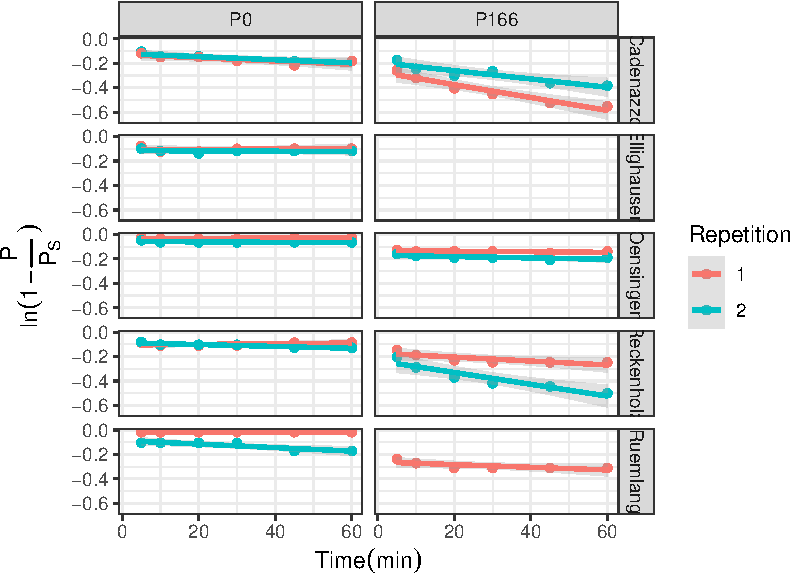
\includegraphics[keepaspectratio]{index_files/figure-pdf/fig-linearized-model-1.pdf}}

}

\caption{\label{fig-linearized-model}Test of the linearized first-order
kinetic model. The plot visually supports the statistical finding that
many intercepts are not zero.}

\end{figure}%

\subsubsection{Final Approach: Successful Non-Linear
Model}\label{final-approach-successful-non-linear-model}

Given the statistical failure of the linearized model, a direct
non-linear modeling approach was adopted to estimate both \(P_{desorb}\)
and \(k\) simultaneously from the untransformed data. This approach does
not rely on the assumption of a zero intercept and proved to be far more
successful, accurately capturing the curvilinear shape of the desorption
data for nearly all samples (Figure~\ref{fig-nonlinear-model}). The
final parameters were extracted from a non-linear mixed-effects model
(\texttt{nlme}) to account for the hierarchical data structure.
\textbf{These final \texttt{nlme}-derived coefficients were used for all
subsequent analyses.}

\phantomsection\label{cell-fig-nonlinear-model}
\begin{figure}[H]

\centering{

\pandocbounded{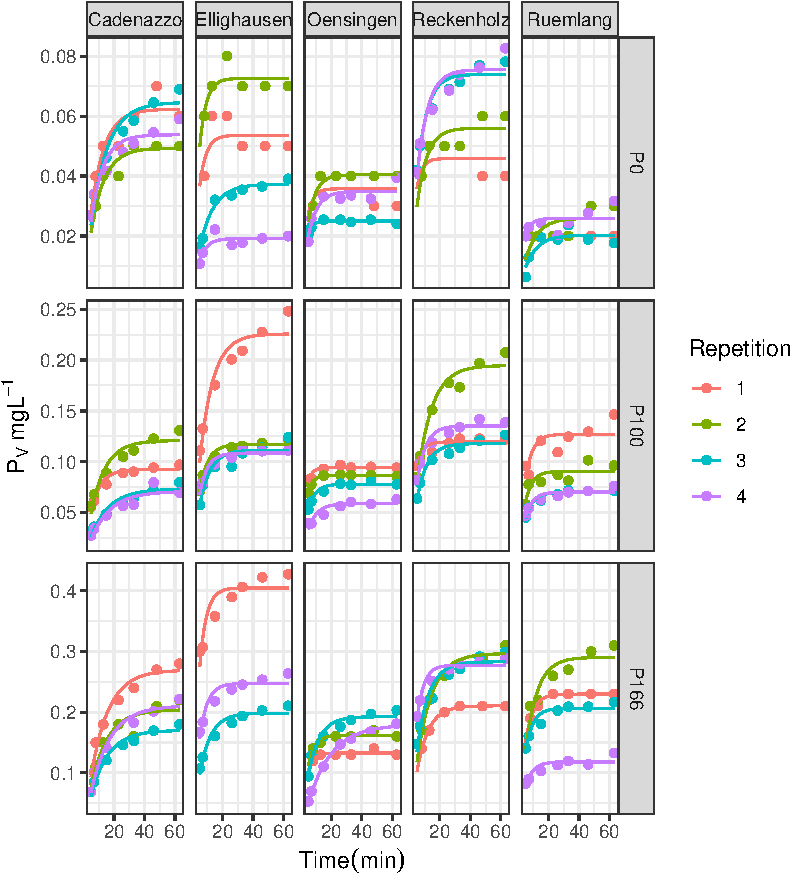
\includegraphics[keepaspectratio]{index_files/figure-pdf/fig-nonlinear-model-1.pdf}}

}

\caption{\label{fig-nonlinear-model}Non-linear first-order kinetic model
fits for P desorption over time. Points represent measured data and
solid lines represent the fitted model for each replicate.}

\end{figure}%

\subsection{Comparison with Isotopic Exchange Kinetics
(IEK)}\label{comparison-with-isotopic-exchange-kinetics-iek}

To validate the newly derived kinetic parameters against an established
benchmark, the capacity (\(P_{desorb}\)) and kinetic (\(k\)) parameters
were compared to data from Isotopic Exchange Kinetics (IEK) studies
previously conducted on the same long-term trial sites by Demaria et
al.~(2013). This comparison aims to determine if the simpler,
non-equilibrium desorption method used in this thesis captures similar
aspects of soil P dynamics as the more complex, equilibrium-based IEK
method.

The size of the desorbable P pool (\(P_{desorb}\)) was compared against
the long-term isotopically exchangeable P pool measured after 7 days
(\(E_{7d}\)). The desorption rate constant (\(k\)) was compared against
the IEK kinetic parameter measured after 24 hours (\(n_{1d}\)).
Spearman's rank correlation was used to robustly test for monotonic
trends between the different methods.

\begin{figure}

\begin{minipage}{0.50\linewidth}

\centering{

\pandocbounded{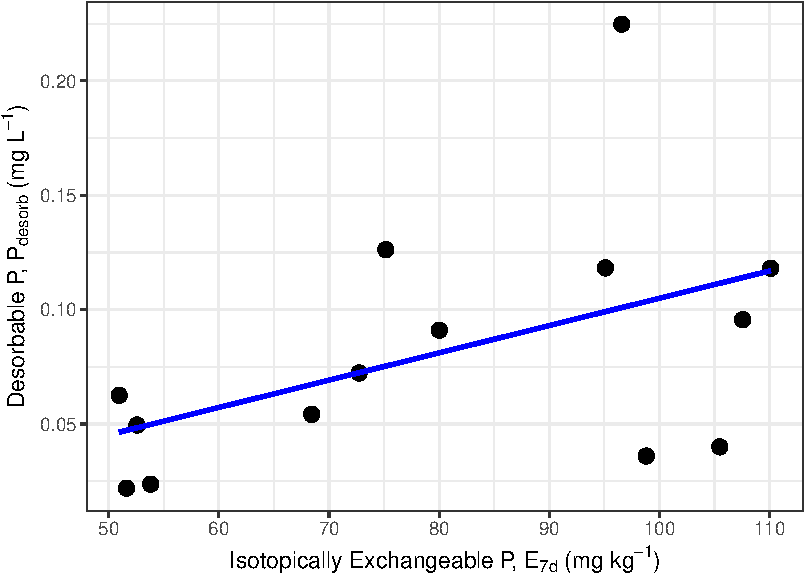
\includegraphics[keepaspectratio]{index_files/figure-pdf/fig-iek-comparison-1.pdf}}

}

\subcaption{\label{fig-iek-comparison-1}Capacity: \(P_{\text{desorb}}\)
vs \(E_{\text{7d}}\)}

\end{minipage}%
%
\begin{minipage}{0.50\linewidth}

\centering{

\pandocbounded{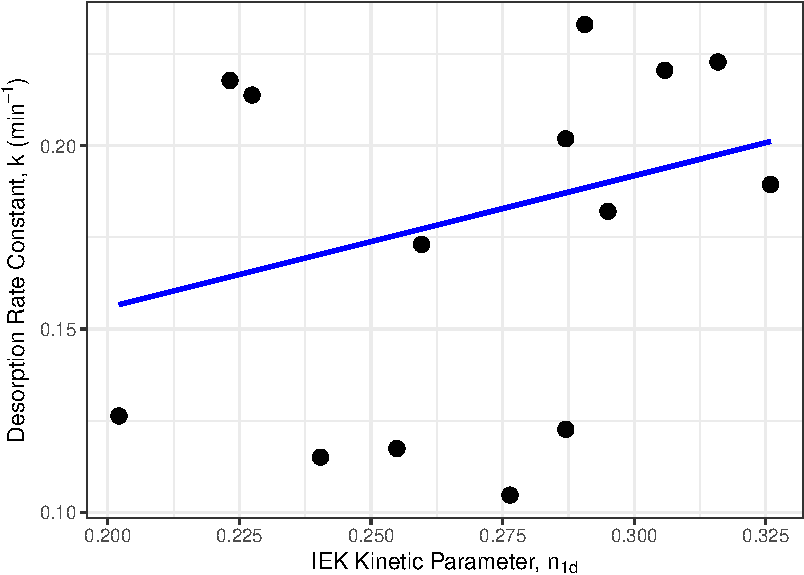
\includegraphics[keepaspectratio]{index_files/figure-pdf/fig-iek-comparison-2.pdf}}

}

\subcaption{\label{fig-iek-comparison-2}Kinetics: k vs
\(n_{\text{1d}}\)}

\end{minipage}%

\caption{\label{fig-iek-comparison}Correlation between
desorption-derived kinetic parameters and IEK-derived parameters. (A)
Capacity parameters: Desorbable P (\(P_{\text{desorb}}\))
vs.~Isotopically Exchangeable P (\(E_{\text{7d}}\)). (B) Kinetic
parameters: Rate Constant (\(k\)) vs.~IEK kinetic parameter
(\(n_{\text{1d}}\)).}

\end{figure}%

The analysis revealed a statistically significant, moderate positive
correlation between the capacity parameters, \(P_{desorb}\) and
\(E_{7d}\) (Figure~\ref{fig-iek-comparison}). The Spearman's rank
correlation coefficient was 0.4 with a p-value of \textless{} 0.001.

Similarly, a statistically significant, moderate positive correlation
was found between the kinetic parameters, \(k\) and \(n_{1d}\)
(Figure~\ref{fig-iek-comparison}). The Spearman's rank correlation
coefficient was 0.36 with a p-value of \textless{} 0.001.

These results indicate that the simpler, non-equilibrium desorption
method used in this study successfully captures both the capacity and
intensity aspects of soil P lability, providing results that are
consistent with the more complex, equilibrium-based IEK method reported
by (Demaria et al., 2013).

\subsection{Effects of Fertilization on Agronomic and Soil
Parameters}\label{sec-effects-of-fertilization-on-agronomic-and-soil-parameters}

Having established a robust method to determine the kinetic parameters,
the next step was to explore the effects of the long-term P
fertilization treatments on both the agronomic outcomes and the soil P
test parameters.

\subsubsection{Agronomic Responses to P
Fertilization}\label{sec-agronomic-responses-to-p-fertilization}

The long-term application of different P fertilization levels had a
pronounced impact on the primary agronomic outcomes, including two
different metrics for yield, P Uptake (\(P_{up}\)), and P Balance
(\(P_{bal}\)), though the response varied considerably between sites
(Figure~\ref{fig-agronomic-responses}).

\phantomsection\label{cell-fig-agronomic-responses}
\begin{figure}[H]

\centering{

\pandocbounded{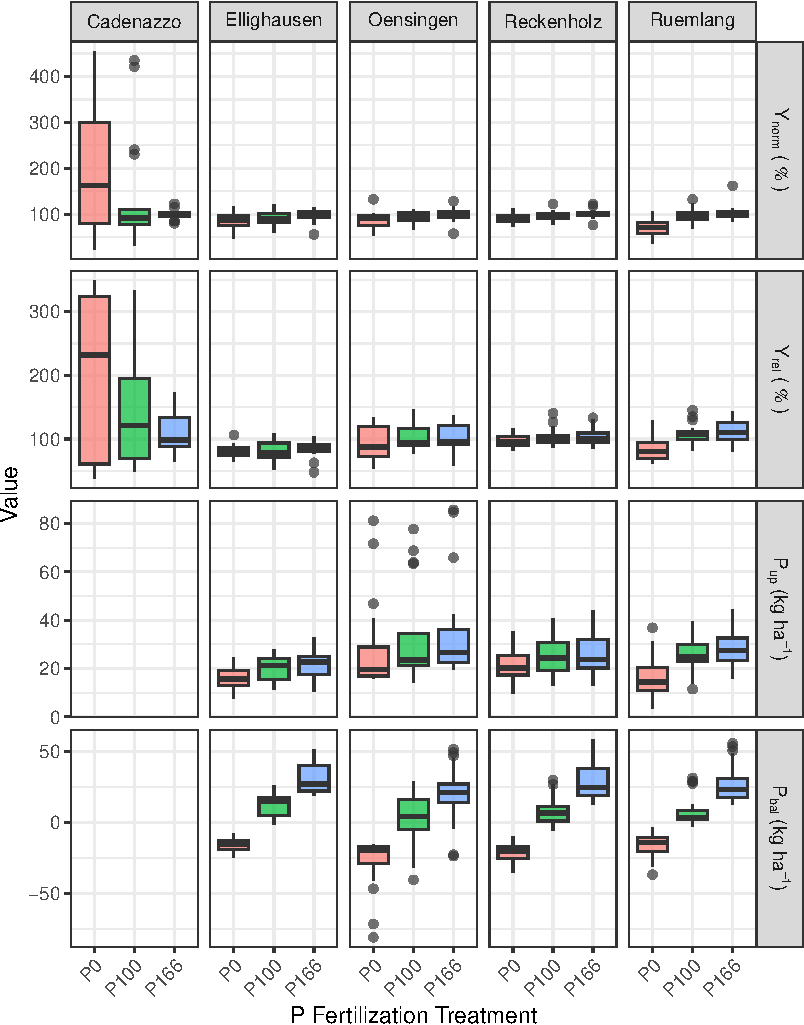
\includegraphics[keepaspectratio]{index_files/figure-pdf/fig-agronomic-responses-1.pdf}}

}

\caption{\label{fig-agronomic-responses}Agronomic response variables
across six P fertilization treatments and six experimental sites. Data
from 2017-2022.}

\end{figure}%

\textbf{Yield Metrics (}\(Y_{norm}\) and \(Y_{rel}\)): Both yield
metrics showed a generally positive response to P fertilization. The
site-normalized yield (\(Y_{norm}\)) shows the response relative to the
site's potential for that year, with most yields plateauing around the
Norm (100\%) treatment. The national-normalized yield (\(Y_{rel}\))
provides a broader context, showing how yields at each site compare to
the national average.

\textbf{P Uptake (}\(P_{up}\)): P uptake by crops followed a similar
trend to yield, increasing with fertilization, often continuing to
increase at the highest fertilization levels, suggesting luxury
consumption.

\textbf{P Balance (}\(P_{bal}\)): The P balance showed a strong, linear
relationship with fertilization. The Zero and Deficit treatments
resulted in a negative balance (mining soil P), while the Elevated and
Surplus treatments led to a significant P surplus.

\subsubsection{Soil P Parameters as a Function of P
Fertilization}\label{sec-soil-p-parameters-as-a-function-of-p-fertilization}

The different soil P test parameters, including the standard STP methods
and the newly derived kinetic parameters, all responded to the long-term
fertilization treatments (Figure~\ref{fig-soil-parameters}).

\phantomsection\label{cell-fig-soil-parameters}
\begin{figure}[H]

\centering{

\pandocbounded{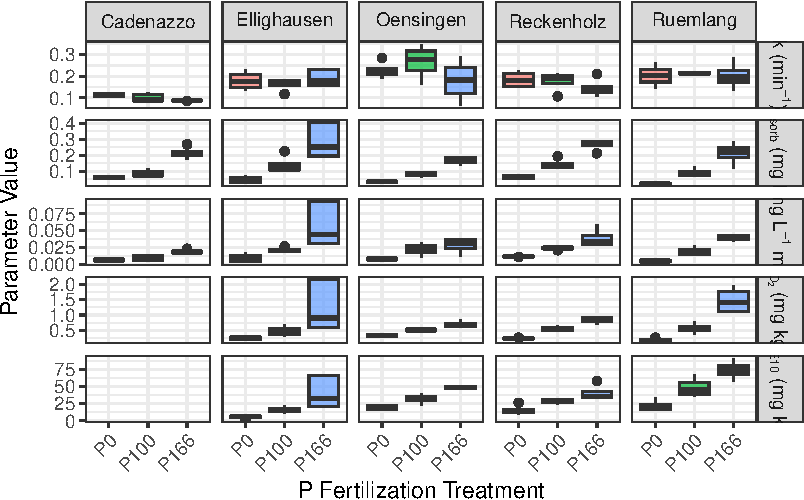
\includegraphics[keepaspectratio]{index_files/figure-pdf/fig-soil-parameters-1.pdf}}

}

\caption{\label{fig-soil-parameters}Soil P parameters across six P
fertilization treatments and six experimental sites.}

\end{figure}%

\textbf{Standard STPs (}\(P_{CO_2}\) and \(P_{AAE10}\)): Both standard
soil P tests showed a clear and consistent increase with rising P
fertilization levels across all sites, confirming their sensitivity to
management.

\textbf{Kinetic Parameters (}\(k\), \(P_{desorb}\), and \(J_0\)):
\textbf{Desorbable P (}\(P_{desorb}\)): This parameter behaved very
similarly to the standard STPs, increasing steadily with P fertilization
and confirming its role as a ``capacity'' indicator.\\
\textbf{Rate Constant (}\(k\)): The rate constant showed a more complex
pattern, with no strong, consistent trend with fertilization. This
suggests that while fertilization increases the \emph{amount} of
available P, it may not change the intrinsic \emph{release rate}.
\textbf{Initial P Flux (}\(J_0\)): As the product of \(P_{desorb}\) and
\(k\), this parameter integrates both capacity and intensity. It showed
a strong positive response to fertilization, driven primarily by the
increase in \(P_{desorb}\).

These initial observations suggest that the kinetic parameters,
particularly the rate constant \(k\), may provide unique information
about the soil's P dynamics not captured by the static tests P-CO2 and
P-AAE10 alone. The next section will use formal statistical models to
test these relationships.

\subsection{Predicting P Parameters from Soil
Properties}\label{sec-p-params-soil-props}

To understand the underlying drivers of the standard and kinetic P
parameters, and to test \textbf{Hypotheses 1b and 2b}, a series of
linear mixed-effects models were fitted. Each model predicted one of the
P parameters based on the core soil properties: organic carbon
(\(C_{org}\)), clay content, silt content, pH, and
dithionite-extractable Al (\(Al_d\)) and Fe (\(Fe_d\)). The results are
summarized in Table~\ref{tbl-soil-prop-models}.

\begin{longtable}[]{@{}
  >{\raggedright\arraybackslash}p{(\linewidth - 10\tabcolsep) * \real{0.1515}}
  >{\raggedright\arraybackslash}p{(\linewidth - 10\tabcolsep) * \real{0.1970}}
  >{\raggedright\arraybackslash}p{(\linewidth - 10\tabcolsep) * \real{0.1515}}
  >{\raggedright\arraybackslash}p{(\linewidth - 10\tabcolsep) * \real{0.1515}}
  >{\raggedright\arraybackslash}p{(\linewidth - 10\tabcolsep) * \real{0.1667}}
  >{\raggedright\arraybackslash}p{(\linewidth - 10\tabcolsep) * \real{0.1818}}@{}}

\caption{\label{tbl-soil-prop-models}Results of linear mixed-effects
models predicting P parameters from intrinsic soil properties
Table~\ref{tbl-variables}. Significance codes: `\emph{\textbf{' p
\textless{} 0.001, '}' p \textless{} 0.01, '}' p \textless{} 0.05.}

\tabularnewline

\toprule\noalign{}
\begin{minipage}[b]{\linewidth}\raggedright
Predictor
\end{minipage} & \begin{minipage}[b]{\linewidth}\raggedright
\(P_{desorb}\)
\end{minipage} & \begin{minipage}[b]{\linewidth}\raggedright
\(k\)
\end{minipage} & \begin{minipage}[b]{\linewidth}\raggedright
\(J_0\)
\end{minipage} & \begin{minipage}[b]{\linewidth}\raggedright
\(P_{CO_2}\)
\end{minipage} & \begin{minipage}[b]{\linewidth}\raggedright
\(P_{AAE10}\)
\end{minipage} \\
\midrule\noalign{}
\endhead
\bottomrule\noalign{}
\endlastfoot
Intercept & 21.444 & 0.454 & 21.189 & 14.014 & 23.126 \\
\(Al_{d}\) & -8.706*** & -0.072*** & -8.631*** & -4.417*** &
-9.473*** \\
\(Fe_{d}\) & -1.068*** & 0.005 & -1.084*** & -0.845*** & -0.606*** \\
Clay & -0.006*** & -0.016*** & -0.085*** & 0.015 & -0.029*** \\
\(C_{org}\) & 0.612 & 0.137 & 1.250 & 0.269 & 1.454 \\
pH & -0.018*** & -0.021*** & -0.092*** & 0.124 & 0.012 \\
Silt & -0.000*** & 0.004 & 0.008 & -0.015*** & -0.049*** \\
\(R^2_m\) & 0.393 & 0.212 & 0.368 & 0.362 & 0.494 \\
\(R^2_c\) & 0.996 & 0.915 & 0.993 & 0.995 & 0.997 \\

\end{longtable}

The analysis reveals that the capacity-based P pools and the kinetic
rate constant are controlled by different sets of soil properties,
strongly supporting the hypotheses.

In line with \textbf{Hypothesis 2b}, the kinetic capacity parameter,
\textbf{Desorbable P (}\(P_{desorb}\)), showed a highly significant
negative relationship with both dithionite-extractable iron (\(Fe_d\))
and aluminum (\(Al_d\)). This provides strong evidence that the total
pool of free oxides, which represent the primary P sorption surfaces in
the soil, is a key factor controlling the size of the readily desorbable
P pool.

Also confirming \textbf{Hypothesis 2b}, the \textbf{Rate Constant
(\emph{k})} was governed by a different set of properties. It was not
significantly influenced by the free oxides but instead showed a
significant negative relationship with \texttt{Clay} content and a
positive relationship with organic carbon (\(C_{org}\)). This clearly
distinguishes the kinetic component from the capacity component,
suggesting that while oxides control \emph{how much} P can be held, soil
texture and organic matter influence \emph{how fast} it can be released.

The standard STP methods showed patterns consistent with
\textbf{Hypothesis 1b}. \textbf{Organic Carbon (}\(C_{org}\)) had a
highly significant positive effect on \(P_{AAE10}\), and \textbf{pH} had
a significant negative effect, as predicted. The relationship of the STP
measures with the dithionite-extractable oxides was less consistent than
that of \(P_{desorb}\), with only \(P_{AAE10}\) showing a significant
negative link to \(Al_d\).

\subsection{Predictive Modeling of Agronomic
Outcomes}\label{sec-agronomic-modeling}

To formally evaluate the predictive power of the standard STP methods
against the kinetic parameters, a series of linear mixed-effects models
were fitted for each of the primary agronomic response variables. To
test the central hypotheses of this thesis, the predictive power of the
kinetic parameters was directly compared against that of the standard
STP methods for several key agronomic outcomes. For each response
variable---Normalized Yield (\(Y_{rel}\)), P Uptake (\(P_{up}\)), and P
Balance (\(P_{bal}\))---a set of competing linear mixed-effects models
was constructed.

To ensure a fair comparison, all models shared an identical random
effects structure
(\texttt{(1\textbar{}year)\ +\ (1\textbar{}Site)\ +\ (1\textbar{}Site:block)}),
differing only in their fixed effects. Four distinct models were
evaluated: \(P_{CO_2}\) Model: Used the standard water-soluble P test as
the sole predictor. \(P_{AAE10}\) Model: Used the standard
chelate-extractable P test as the sole predictor. \textbf{STP
Interaction Model:} Included both standard tests and their interaction
term (\(P_{CO_2} * P_{AAE10}\)) to capture their combined effect.
\textbf{Kinetic Model:} Used the log-transformed desorbable P pool
(\(log(P_{desorb})\)), the rate constant (\emph{k}), and their
interaction (\(J_0\)) as predictors.

The performance of these models for each agronomic outcome is presented
in the following sections.

\subsubsection{Anomaly in the Cadenazzo Yield
Data}\label{anomaly-in-the-cadenazzo-yield-data}

A preliminary visual analysis of the agronomic data revealed a
significant anomaly at the Cadenazzo (CAD) site. As shown in
Figure~\ref{fig-yield-comparison}, the Cadenazzo site exhibited
substantially higher overall yields than all other locations. More
critically, the yield response to P fertilization did not follow the
expected agronomic trend. The zero-fertilizer treatment (\texttt{P0})
showed the highest median yield, while the surplus treatment
(\texttt{P166}) was among the lowest.

A simple label swap between \texttt{P0} and \texttt{P166} was
hypothesized and tested (Figure~\ref{fig-yield-cadenazzo-fix}). While
this correction established a more monotonic trend, the resulting
pattern remained questionable, with the corrected \texttt{P166} yield
being inexplicably higher than the \texttt{P100} and \texttt{P133}
treatments, which is not a typical biological response.

Unfortunately, a deeper investigation into the cause of this anomaly was
impossible, as the corresponding soil analysis data (STPs, organic
carbon, etc.) for the Cadenazzo site were unavailable due to sample
loss. Without this data, it cannot be determined whether the issue stems
from a persistent micro-site anomaly, a more complex data recording
error, or other unknown factors. Given these unresolved inconsistencies
and the site's unusually high productivity, the Cadenazzo data was
retained in the models but is recognized as a significant source of
unexplained variance that likely contributed to the poor predictive
performance of all models for yield-related metrics like \(Y_{norm}\)
and \(Y_{rel}\).

\phantomsection\label{cell-fig-yield-comparison}
\begin{figure}[H]

\centering{

\pandocbounded{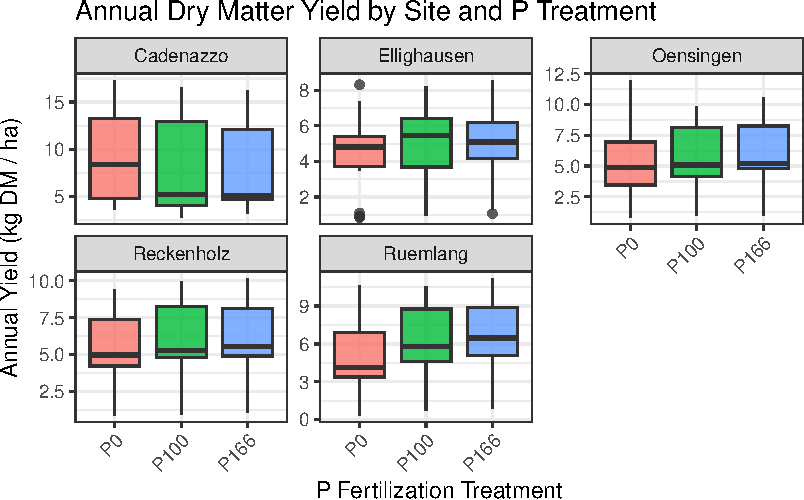
\includegraphics[keepaspectratio]{index_files/figure-pdf/fig-yield-comparison-1.pdf}}

}

\caption{\label{fig-yield-comparison}Annual dry matter yield across P
fertilization treatments, faceted by experimental site, highlighting the
anomalous pattern at Cadenazzo (CAD).}

\end{figure}%

\phantomsection\label{cell-fig-yield-cadenazzo-fix}
\begin{figure}[H]

\centering{

\pandocbounded{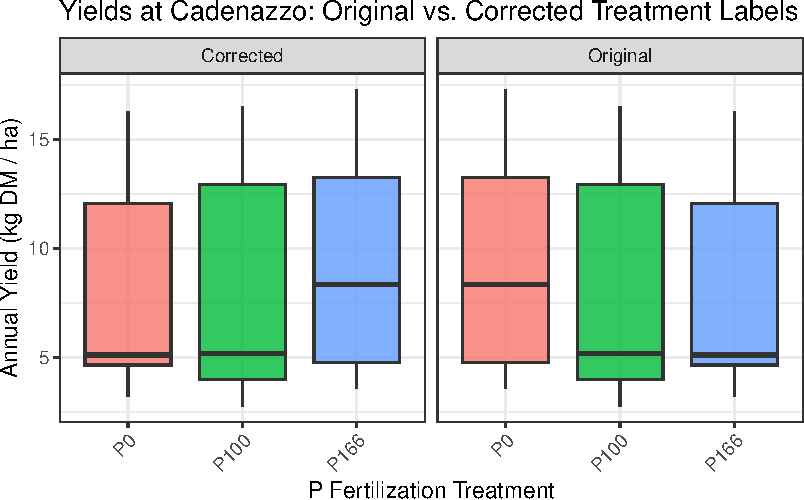
\includegraphics[keepaspectratio]{index_files/figure-pdf/fig-yield-cadenazzo-fix-1.pdf}}

}

\caption{\label{fig-yield-cadenazzo-fix}Comparison of Cadenazzo yields
with original and swapped (P0 \textless\textgreater{} P166) treatment
labels.}

\end{figure}%

\subsubsection{\texorpdfstring{Predicting Site-Normalized Yield
(\(Y_{norm}\))}{Predicting Site-Normalized Yield (Y\_\{norm\})}}\label{predicting-site-normalized-yield-y_norm}

The analysis reveals a clear and striking difference between the
predictive power of the standard STP methods and the kinetic parameters
for site-normalized yield, as seen in Table~\ref{tbl-ynorm-models}.

\begin{longtable}[]{@{}
  >{\raggedright\arraybackslash}p{(\linewidth - 8\tabcolsep) * \real{0.3733}}
  >{\raggedright\arraybackslash}p{(\linewidth - 8\tabcolsep) * \real{0.1467}}
  >{\raggedright\arraybackslash}p{(\linewidth - 8\tabcolsep) * \real{0.1600}}
  >{\raggedright\arraybackslash}p{(\linewidth - 8\tabcolsep) * \real{0.2133}}
  >{\raggedright\arraybackslash}p{(\linewidth - 8\tabcolsep) * \real{0.1067}}@{}}

\caption{\label{tbl-ynorm-models}Results of linear mixed-effects models
predicting Site-Normalized Yield (\(Y_{norm}\)).}

\tabularnewline

\toprule\noalign{}
\begin{minipage}[b]{\linewidth}\raggedright
Predictor
\end{minipage} & \begin{minipage}[b]{\linewidth}\raggedright
\(P_{CO_2}\)
\end{minipage} & \begin{minipage}[b]{\linewidth}\raggedright
\(P_{AAE10}\)
\end{minipage} & \begin{minipage}[b]{\linewidth}\raggedright
STP-interaction
\end{minipage} & \begin{minipage}[b]{\linewidth}\raggedright
kinetic
\end{minipage} \\
\midrule\noalign{}
\endhead
\bottomrule\noalign{}
\endlastfoot
Intercept & 1.059*** & 0.532*** & 1.096*** & 0.980 \\
\(k\) & & & & 2.262 \\
\(J_0\) & & & & 0.931 \\
\(P_{desorb}\) & & & & -0.063 \\
\(P_{AAE10}\) & & 0.120*** & -0.006 & \\
\(P_{CO_2}\) & 0.162*** & & 0.137 & \\
\(P_{CO_2} \times P_{AAE10}\) & & & 0.016 & \\
\(R^2_m\) & 0.218 & 0.198 & 0.220 & 0.014 \\
\(R^2_c\) & 0.358 & 0.474 & 0.365 & 0.360 \\

\end{longtable}

The analysis for site-normalized yield showed that both the
\texttt{\$P\_\{CO\_2\}\$} and \texttt{\$P\_\{AAE10\}\$} models had
highly significant coefficients and explained 21.8\% and 19.8\% of the
variance, respectively. The combined STP-interaction model performed
best, explaining 22\% of the variance. In contrast, the kinetic model
had a marginal R² of only 1.4\%, and none of its parameters were
statistically significant.

\subsubsection{\texorpdfstring{Predicting National-Normalized Yield
(\(Y_{rel}\))}{Predicting National-Normalized Yield (Y\_\{rel\})}}\label{predicting-national-normalized-yield-y_rel}

The models predicting national-normalized yield (\(Y_{rel}\)) reveal
that both standard and kinetic soil phosphorus tests struggle to explain
the variance in crop yields on their own, though standard tests show
slightly better performance in this context.

\begin{longtable}[]{@{}
  >{\raggedright\arraybackslash}p{(\linewidth - 8\tabcolsep) * \real{0.3636}}
  >{\raggedright\arraybackslash}p{(\linewidth - 8\tabcolsep) * \real{0.1429}}
  >{\raggedright\arraybackslash}p{(\linewidth - 8\tabcolsep) * \real{0.1558}}
  >{\raggedright\arraybackslash}p{(\linewidth - 8\tabcolsep) * \real{0.2078}}
  >{\raggedright\arraybackslash}p{(\linewidth - 8\tabcolsep) * \real{0.1299}}@{}}

\caption{\label{tbl-yrel-models}Results of linear mixed-effects models
predicting National-Normalized Yield (\(Y_{rel}\)).}

\tabularnewline

\toprule\noalign{}
\begin{minipage}[b]{\linewidth}\raggedright
Predictor
\end{minipage} & \begin{minipage}[b]{\linewidth}\raggedright
\(P_{CO_2}\)
\end{minipage} & \begin{minipage}[b]{\linewidth}\raggedright
\(P_{AAE10}\)
\end{minipage} & \begin{minipage}[b]{\linewidth}\raggedright
STP-interaction
\end{minipage} & \begin{minipage}[b]{\linewidth}\raggedright
kinetic
\end{minipage} \\
\midrule\noalign{}
\endhead
\bottomrule\noalign{}
\endlastfoot
Intercept & 104.862*** & 75.343*** & 130.274*** & 56.375 \\
\(k\) & & & & 377.498** \\
\(J_0\) & & & & 171.507** \\
\(P_{desorb}\) & & & & -27.486* \\
\(P_{AAE10}\) & & 7.111** & -6.537 & \\
\(P_{CO_2}\) & 8.853** & & 23.091 & \\
\(P_{CO_2} \times P_{AAE10}\) & & & -3.110 & \\
\(R^2_m\) & 0.074 & 0.063 & 0.078 & 0.022 \\
\(R^2_c\) & 0.569 & 0.537 & 0.596 & 0.439 \\

\end{longtable}

\paragraph{Performance of Standard STP
Methods}\label{performance-of-standard-stp-methods}

The models based on standard soil tests, \texttt{\$P\_\{CO\_2\}\$} and
\texttt{\$P\_\{AAE10\}\$}, were significant predictors, explaining 7.4\%
and 6.3\% of the variance in yield, respectively. The model including
their interaction term performed slightly better, explaining 7.8\% of
the variance. The model based on kinetic parameters demonstrated lower
predictive power, with a marginal R² of 2.2\%. A critical observation
across all models is the large discrepancy between the marginal R²
(\(R^2_m\)) and the conditional R² (\(R^2_c\)). For instance, in the
best-performing STP model, the marginal R² is only 0.078, but the
conditional R² is 0.596.

\subsubsection{\texorpdfstring{Predicting P-Uptake
(\(P_{up}\))}{Predicting P-Uptake (P\_\{up\})}}\label{predicting-p-uptake-p_up}

When predicting P-uptake, both the standard and kinetic models
demonstrate similarly weak predictive power, with none of the approaches
standing out as superior.

\begin{longtable}[]{@{}
  >{\raggedright\arraybackslash}p{(\linewidth - 8\tabcolsep) * \real{0.3636}}
  >{\raggedright\arraybackslash}p{(\linewidth - 8\tabcolsep) * \real{0.1429}}
  >{\raggedright\arraybackslash}p{(\linewidth - 8\tabcolsep) * \real{0.1558}}
  >{\raggedright\arraybackslash}p{(\linewidth - 8\tabcolsep) * \real{0.2078}}
  >{\raggedright\arraybackslash}p{(\linewidth - 8\tabcolsep) * \real{0.1299}}@{}}

\caption{\label{tbl-pexport-models}Results of linear mixed-effects
models predicting P-Export (\(P_{up}\)).}

\tabularnewline

\toprule\noalign{}
\begin{minipage}[b]{\linewidth}\raggedright
Predictor
\end{minipage} & \begin{minipage}[b]{\linewidth}\raggedright
\(P_{CO_2}\)
\end{minipage} & \begin{minipage}[b]{\linewidth}\raggedright
\(P_{AAE10}\)
\end{minipage} & \begin{minipage}[b]{\linewidth}\raggedright
STP-interaction
\end{minipage} & \begin{minipage}[b]{\linewidth}\raggedright
kinetic
\end{minipage} \\
\midrule\noalign{}
\endhead
\bottomrule\noalign{}
\endlastfoot
Intercept & 27.522*** & 8.090 & 30.632* & 29.599*** \\
\(k\) & & & & 22.622 \\
\(J_0\) & & & & 11.928 \\
\(P_{desorb}\) & & & & 1.954 \\
\(P_{AAE10}\) & & 4.824*** & -0.805 & \\
\(P_{CO_2}\) & 5.177*** & & 8.069 & \\
\(P_{CO_2} \times P_{AAE10}\) & & & -0.814 & \\
\(R^2_m\) & 0.064 & 0.073 & 0.065 & 0.064 \\
\(R^2_c\) & 0.625 & 0.603 & 0.623 & 0.648 \\

\end{longtable}

When predicting P-uptake, the individual standard soil tests,
\(P_{CO_2}\) and \(P_{AAE10}\), were significant positive predictors,
explaining 6.4\% and 7.3\% of the variance, respectively. The
interaction model did not improve the explained variance. The kinetic
model performed on par with the standard individual tests, explaining
6.4\% of the variance, though none of its parameters were individually
significant. As with yield, a large difference between the marginal and
conditional R² values was observed across all models.

\subsubsection{\texorpdfstring{Predicting P-Balance
(\(P_{bal}\))}{Predicting P-Balance (P\_\{bal\})}}\label{predicting-p-balance-p_bal}

The prediction of the P-Balance (\(P_{bal}\)) reveals a stark and
decisive contrast between the kinetic and standard STP approaches,
providing the strongest evidence in favor of the kinetic methodology.

\begin{longtable}[]{@{}
  >{\raggedright\arraybackslash}p{(\linewidth - 8\tabcolsep) * \real{0.3636}}
  >{\raggedright\arraybackslash}p{(\linewidth - 8\tabcolsep) * \real{0.1429}}
  >{\raggedright\arraybackslash}p{(\linewidth - 8\tabcolsep) * \real{0.1558}}
  >{\raggedright\arraybackslash}p{(\linewidth - 8\tabcolsep) * \real{0.2078}}
  >{\raggedright\arraybackslash}p{(\linewidth - 8\tabcolsep) * \real{0.1299}}@{}}

\caption{\label{tbl-pbalance-models}Results of linear mixed-effects
models predicting P-Balance (\(P_{bal}\)).}

\tabularnewline

\toprule\noalign{}
\begin{minipage}[b]{\linewidth}\raggedright
Predictor
\end{minipage} & \begin{minipage}[b]{\linewidth}\raggedright
\(P_{CO_2}\)
\end{minipage} & \begin{minipage}[b]{\linewidth}\raggedright
\(P_{AAE10}\)
\end{minipage} & \begin{minipage}[b]{\linewidth}\raggedright
STP-interaction
\end{minipage} & \begin{minipage}[b]{\linewidth}\raggedright
kinetic
\end{minipage} \\
\midrule\noalign{}
\endhead
\bottomrule\noalign{}
\endlastfoot
Intercept & 4.441 & 7.691 & 3.649 & 43.833*** \\
\(k\) & & & & 84.993 \\
\(J_0\) & & & & 33.029 \\
\(P_{desorb}\) & & & & 16.947*** \\
\(P_{AAE10}\) & & -0.794 & 0.187 & \\
\(P_{CO_2}\) & -0.928 & & -2.442 & \\
\(P_{CO_2} \times P_{AAE10}\) & & & 0.462 & \\
\(R^2_m\) & 0.001 & 0.001 & 0.001 & 0.572 \\
\(R^2_c\) & 0.810 & 0.807 & 0.811 & 0.744 \\

\end{longtable}

The kinetic model emerged as a strong predictor of the P-Balance,
explaining 57.2\% of the variance, with the desorbable P pool
(\(P_{desorb}\)) being a highly significant predictor. In contrast, all
models based on the standard STP methods had marginal R² values of 0.1\%
and no significant predictors. The conditional R² for the STP models was
high (around 0.81), while the kinetic model had both a high marginal R²
(0.572) and a high conditional R² (0.744).

\newpage

\section{Discussion}\label{discussion}

Before addressing the individual hypotheses, it is crucial to first
evaluate the overall feasibility of the experimental results and the
integrity of the underlying data. A critical examination of the
agronomic data revealed a significant and implausible anomaly at the
Cadenazzo (CAD) site. Across multiple years, the zero-fertilizer
treatment (\texttt{P0}), which has not received P for nearly 40 years,
consistently showed higher median yields than the optimally fertilized
treatments. This contradicts fundamental agronomic principles and stands
in contrast to previous findings from the same long-term experiment
(Hirte, Richner, et al., 2021), suggesting a systematic issue with the
data from this specific site. As the corresponding soil analysis data
for Cadenazzo was unavailable, a definitive explanation for this anomaly
could not be found. This unresolved issue, combined with the site's
uniquely high productivity, introduces significant unexplained variance
and must be considered when interpreting the performance of the
predictive models, particularly for yield-based metrics.

A second key observation is the consistent, large discrepancy between
the marginal R-squared (\(R^2_m\)) and conditional R-squared (\(R^2_c\))
values in the models for yield and P-uptake. This finding is plausible
and expected, as it underscores that in P-sufficient Swiss soils, crop
yield is primarily co-limited by overarching pedoclimatic factors rather
than P availability alone. The Swiss fertilization guidelines (GRUD), on
which the \texttt{P100} treatment is based, were designed to ensure P is
never limiting, which over decades has led to a widespread accumulation
of ``legacy P'' in many agricultural soils (Hirte et al., 2018).
Consequently, the \texttt{P100} and \texttt{P166} treatments in this
study were likely operating in a P-surplus range, well above the
critical threshold for a yield response. This lack of P-limitation means
the experiment was not designed to effectively test the sensitivity of
different soil P metrics for predicting yield, which fundamentally
influences the size and significance of the effects we could detect.

Therefore, a marginal R² of around 8\% for a model predicting
national-normalized yield based on a single soil P metric should not be
considered low. In fact, it is arguably higher than expected,
demonstrating that despite the overwhelming influence of climate and the
general P-sufficiency of the soils, both static and kinetic P tests can
still capture a statistically significant, albeit small, portion of the
variance in crop productivity. With this context established, we can
proceed to a detailed evaluation of the specific hypotheses.

\subsection{Hypothesis 1: The Nuanced Role of Standard Soil
Tests}\label{hypothesis-1-the-nuanced-role-of-standard-soil-tests}

\textbf{Hypothesis 1a} posited that standard STP methods (\(P_{CO_2}\)
and \(P_{AAE10}\)) would correlate with the P-Balance but be weak
predictors of crop yield. The findings challenge this hypothesis in two
unexpected ways.

First, the STP methods \textbf{failed completely to predict the
P-Balance}. The models showed no relationship between these static tests
and the long-term nutrient surplus or deficit, directly contradicting
our hypothesis. This is a critical finding, as it suggests that while
tests like \(P_{CO_2}\) and \(P_{AAE10}\) are sensitive to short-term
changes from annual fertilization, they do not adequately capture the
cumulative, long-term P status of the soil system.

Second, the performance of STP methods in predicting yield was highly
context-dependent. When predicting \textbf{site-normalized yield
(}\(Y_{norm}\)), which assesses the yield response relative to a site's
own potential, the STP models were remarkably effective, explaining up
to 22\% of the variance. This result contradicts the part of our
hypothesis that expected weak performance and suggests that for
\emph{within-field} management, where the goal is to ensure P is not
limiting relative to that specific environment's potential, traditional
capacity-based tests are well-suited and robust.

However, when predicting \textbf{national-normalized yield
(}\(Y_{rel}\)) and \textbf{P-uptake (}\(P_{up}\)), the STP models
performed poorly, aligning with our initial expectations. The weak
performance in predicting yield and P-uptake can likely be attributed to
several factors. Firstly, crop yield in field settings is often
co-limited by multiple factors beyond phosphorus. Year-to-year
variations in climate, such as solar radiation and water availability,
as well as the supply of other key nutrients like nitrogen, can become
the primary drivers of productivity, masking the more subtle influence
of soil P status (Sadras, 2002; Sinclair, 1998). The large gap between
the marginal and conditional \(R^2\) in our models strongly suggests
that these site- and year-specific variables, captured by the random
effects, were indeed the dominant factors.

Furthermore, response variables like \(P_{up}\) and \(P_{bal}\) are
calculated as the product of yield and P concentration, which can
introduce and propagate measurement uncertainty. If yield itself is only
weakly correlated with soil P status, this ``noise'' is carried into the
derived variables, making it even more difficult to establish a clear
statistical relationship (Rowe et al., 2016).

The predictive weakness may also stem from the experimental design and
modeling approach. This study utilized samples primarily from the
P-deficient (0\%) and P-sufficient (100\% and 167\%) treatments. Crop
yield response to fertilizer typically follows a saturation curve, and
it is possible that our dataset was concentrated on the less responsive
parts of this curve, thus lacking statistical power in the most dynamic
range (Schlesinger, 2009). While our use of a linear mixed-effects model
was appropriate for the available data, it cannot capture the
diminishing returns characteristic of crop nutrient response. As
demonstrated by \textbf{Hirte et al.~(2021)} on these same STYCS trials,
non-linear models like the Mitscherlich equation are better suited for
describing such saturation kinetics but would require data from the
intermediate fertilization levels to be applied robustly (Hirte,
Stüssel, et al., 2021).

Regarding \textbf{Hypothesis 1b}, the findings were largely supportive.
The analysis of soil properties confirmed that STP measurements are not
pure measures of P but are instead complex indices reflecting a
combination of P status and overarching soil chemistry. The predicted
negative relationship between \textbf{pH} and \(P_{AAE10}\) was
observed, and the underlying chemical mechanisms for this are
well-established, particularly in calcareous or high-pH soils like
several in this study (e.g., ALT, GRA).

The AAE10 method relies on two key components: ammonium acetate as a
buffer and EDTA as a chelating agent to dissolve mineral-bound P.
However, its effectiveness is compromised in soils with high pH and an
abundance of free calcium (\(Ca^{2+}\)) and magnesium (\(Mg^{2+}\))
cations, often from calcium carbonates (\(CaCO_3\)). There are two
primary reasons for this:

\begin{enumerate}
\def\labelenumi{\arabic{enumi}.}
\tightlist
\item
  \textbf{Consumption of EDTA:} The primary role of EDTA is to bind to
  cations like iron and aluminum that precipitate phosphate, thereby
  releasing P into the solution. However, EDTA has a high affinity for
  divalent cations, so in calcareous soils, a significant portion of the
  EDTA is consumed by binding to the abundant free \(Ca^{2+}\) and
  \(Mg^{2+}\), making it less available to extract the target phosphate
  compounds (Fixen \& Grove, 1993).
\item
  \textbf{Buffering Capacity:} The acetate buffer in the AAE10 solution
  is designed to maintain a consistent pH. However, soils with high
  carbonate content have a strong natural buffering capacity that can
  resist the pH change intended by the extractant, further reducing its
  efficiency in dissolving pH-sensitive P minerals.
\end{enumerate}

This known limitation explains why \(P_{AAE10}\) can underestimate
plant-available P in calcareous soils and supports our finding of a
significant pH-dependence. It underscores that the choice of an
appropriate soil test must take into account the fundamental chemistry
of the soil matrix itself.

\subsection{Hypothesis 2: Characterizing P Desorption
Kinetics}\label{hypothesis-2-characterizing-p-desorption-kinetics}

\textbf{Hypothesis 2a} focused on the methodological feasibility of
characterizing P desorption. It predicted that while the process would
follow first-order kinetics, a non-linear modeling approach would be
more robust than the original linearized method proposed by Flossmann \&
Richter (1982). The results from this thesis unequivocally support this
hypothesis. Our initial attempts to linearize the desorption data failed
systematically, with model intercepts deviating significantly from the
required origin, thus violating a core assumption of the method.

This statistical failure has a fundamental chemical basis. The
linearized model requires an \emph{a priori} estimate of the maximum
desorbable P pool (\(P_{desorb}\)), which Flossmann and Richter
approximated by subtracting a water-soluble P measurement from a
stronger chemical extractant (e.g.,
\(P_{desorb} \approx P_{CAL} - P_{H2O}\)). However, in all but the most
severely depleted soils, the P value from the stronger extractant is
orders of magnitude greater than that from water
(\(P_{CAL} >> P_{H2O}\)). This leads to an estimated \(P_{desorb}\) that
is vastly higher than the actual solubility limit of phosphate in the
soil solution. A kinetic desorption curve in water can physically only
plateau at the concentration dictated by mineral solubility; by
providing the model with a theoretical maximum that is chemically
unattainable, the linearization becomes mathematically invalid. This
explains why the linearized approach failed and underscores the
necessity of a method that does not rely on such flawed assumptions.

In contrast, the direct application of a non-linear mixed-effects model
successfully captured the curvilinear nature of P release for nearly all
samples by estimating \(P_{desorb}\) directly from the kinetic data
itself. This confirms that while the foundational concept of first-order
kinetics is sound, modern computational methods that avoid data
transformation provide a far more accurate and statistically valid
approach to parameter estimation (Kuang et al., 2012).

While the non-linear model proved robust, visual inspection of the
kinetic curves revealed that two specific replicates---from the P100 and
P166 treatments at the Ellighausen site---showed markedly higher and
faster P release than their counterparts. To determine whether this was
due to a methodological artifact or true field variability, the standard
soil test results for all replicates at this site were examined
(Figure~\ref{fig-ell-outlier-check-dual-axis}). The diagnostic plot
clearly shows that these same two replicates also registered as
significant outliers for both \(P_{CO_2}\) and \(P_{AAE10}\). This
consistent pattern across three independent measurement techniques
strongly suggests that the deviation is not a result of error in the
kinetic procedure, but rather reflects genuine \textbf{micro-site
heterogeneity}.

Such heterogeneity could arise from several sources. One plausible
explanation, given the decades-long application of Triple-Superphosphate
(primarily monocalcium phosphate), is the presence of residual,
undissolved fertilizer granules in the soil matrix. The accidental
inclusion of even a single such particle in the 10g subsample for a
specific replicate would lead to artificially inflated P values across
all chemical extractions (Fisher, 1925). This highlights a fundamental
challenge in soil analysis and reinforces the importance of robust
modeling. The use of a non-linear \emph{mixed-effects} model is
particularly advantageous in this context, as it is designed to handle
such individual variations by estimating a common overall trend while
allowing for random deviations for each sample, thereby preventing a few
anomalous data points from unduly influencing the overall conclusions
{[}Fisher (1925); Fisher1935; Yates1964; Van Es et al. (2002){]}.

Ultimately, the successful validation of our derived parameters against
established Isotopic Exchange Kinetic (IEK) data further solidifies the
robustness of our methodological approach, demonstrating that this
simpler extraction method effectively captures both the capacity
(\(P_{desorb}\)) and intensity (\emph{k}) aspects of P dynamics.

\phantomsection\label{cell-fig-ell-outlier-check-dual-axis}
\begin{figure}[H]

\centering{

\pandocbounded{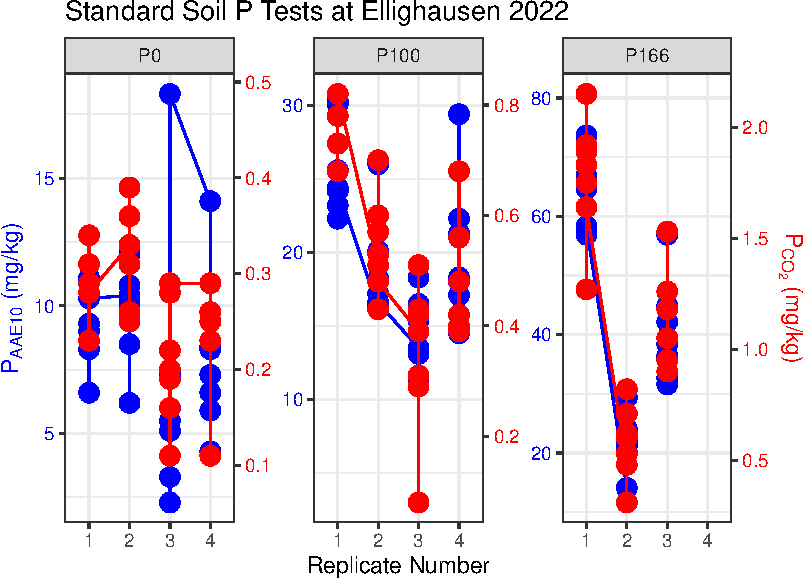
\includegraphics[keepaspectratio]{index_files/figure-pdf/fig-ell-outlier-check-dual-axis-1.pdf}}

}

\caption{\label{fig-ell-outlier-check-dual-axis}Diagnostic plot for
\(P_{\text{AAE10}}\) (left axis) and \(P_{\text{CO2}}\) (right axis) for
all replicates at the Ellighausen (ELL) site, faceted by P fertilization
treatment.}

\end{figure}%

\textbf{Hypothesis 2b} predicted that the derived kinetic parameters
would be significantly influenced by fundamental soil properties, and
this was also strongly supported by the findings. The analysis revealed
a clear and meaningful separation in the drivers of the capacity and
kinetic components. The desorbable P pool (\(P_{desorb}\)), representing
the quantity of readily available P, was strongly and negatively
correlated with dithionite-extractable iron and aluminum. This aligns
perfectly with established soil science principles, as these free oxides
provide the primary sorption surfaces that bind P, thereby controlling
the size of the exchangeable pool (Brady \& Weil, 2016; Sposito, 2008).

Conversely, the rate constant (\emph{k}), which represents the speed of
P release, was not primarily driven by the oxide content but was instead
significantly related to soil texture (clay content) and pH. The
negative relationship with clay content is logical, as higher clay
content can increase the tortuosity of diffusion pathways, effectively
slowing the movement of phosphate from the solid phase to the bulk
solution (Nye \& Tinker, 2000). The influence of pH is also consistent
with known phosphate chemistry, as pH governs the speciation of
orthophosphate ions and their affinity for mineral surfaces (Sparks,
2003). These distinct relationships confirm that \(P_{desorb}\) and
\emph{k} are not redundant parameters; they represent fundamentally
different aspects of P availability---the size of the pool and the rate
of access to it---which are governed by different soil-chemical and
physical properties.

\subsection{Hypothesis 3: The Context-Dependent Power of Kinetic
Parameters}\label{hypothesis-3-the-context-dependent-power-of-kinetic-parameters}

The central hypothesis of this thesis predicted that a model
incorporating kinetic parameters (\emph{k} and \(P_{desorb}\)) would
explain a significantly greater proportion of the variance in agronomic
outcomes compared to models based on standard, static STP measurements.
The results provide a nuanced verdict: the hypothesis was strongly
supported in one context, but clearly refuted in others, revealing that
the utility of kinetic parameters is highly dependent on the specific
agronomic question being addressed.

The most compelling support for \textbf{Hypothesis 3} came from the
prediction of the \textbf{P-Balance (}\(P_{bal}\)). In this analysis,
the kinetic model, driven by the desorbable P pool (\(P_{desorb}\)), was
exceptionally powerful, explaining over 57\% of the variance. In stark
contrast, the standard STP models had zero predictive power. This is the
most significant finding of this study. The P-Balance represents the
long-term integration of nutrient inputs and outputs, and the fact that
a kinetic capacity parameter (\(P_{desorb}\)) so perfectly captures this
state demonstrates its superiority for assessing the cumulative effects
of soil management. It suggests that while standard tests reflect the
immediate chemical environment, \(P_{desorb}\) provides a more holistic
measure of the soil's P supply capacity and its legacy from past
fertilization.

However, when predicting yield and P-uptake, the hypothesis was not
supported. The reasons for this are likely multifaceted and highlight
several limitations of the current study. A primary factor is that the P
fertilization levels analyzed (0\%, 100\%, and 167\%) may not have
created conditions where P was the primary limiting factor for yield.
The standard 100\% fertilization rate in the STYCS trial is already
designed for optimal yield, and decades of application at this level
have likely led to significant ``legacy P'' accumulation (Hirte et al.,
2018). Consequently, the 167\% treatment would only add to this surplus,
while the 0\% treatment represents an extreme deficiency. A direct
comparison between kinetic and static tests would be far more powerful
if intermediate levels (e.g., 33\% and 67\%) were included, as this is
the range where the \emph{rate} of P supply is most likely to be a
yield-limiting factor.

Furthermore, the linear mixed-effects models used, while appropriate for
the data structure, could not account for two major sources of
variation. First, as seen in the exploratory analysis in with the
mlr3-model-comparisons, weather variables alone were often strong
predictors of yield. The \texttt{(1\textbar{}year)} and
\texttt{(1\textbar{}Site)} random effects in our models are proxies for
this, bundling complex pedoclimatic information---such as growing degree
days, soil moisture patterns, and soil textural differences---into
single terms. These effects were so large that they overshadowed the
more subtle influence of soil P status. Future studies could improve
predictive power by incorporating specific weather covariates as fixed
effects, allowing for a clearer isolation of the soil P signal.

Second, the assumption of a linear P response is a simplification. As
shown by \textbf{Hirte et al.~(2021)}, crop yield response to P is
non-linear and best described by a saturation curve. This is
particularly relevant given the high yields observed at some sites, such
as Cadenazzo, where relative yields reached up to 300\% in some years, a
level far beyond any plausible linear response to P. A more robust
modeling approach would involve fitting non-linear models, though this
would, as previously noted, require data from the full spectrum of
fertilization treatments.

\newpage

\subsubsection{Conclusion and Outlook}\label{conclusion-and-outlook}

This thesis set out to test the hypothesis that P desorption kinetics,
grounded in the diffusion-limited reality of P uptake, would provide a
superior prediction of agronomic outcomes compared to conventional
static soil tests (STPs). The first step required a critical
re-evaluation of the kinetic methodology itself. We successfully
demonstrated that the original linearized approach of Flossmann \&
Richter (1982) is based on a chemically flawed premise, where the
estimated desorbable P pool (\(P_{desorb}\)) far exceeds the physical
solubility of phosphate. By implementing a direct non-linear modeling
approach, we derived robust kinetic parameters free from these
assumptions. However, this refined method remains sensitive, as
evidenced by outlier replicates that were ultimately attributed to the
``nugget effect'' of residual fertilizer granules, a persistent
challenge in soil analysis.

The comparative analysis of the predictive models yielded a nuanced
picture. Contrary to our primary hypothesis, the kinetic parameters were
not universally superior. For predicting site- and national-normalized
yield (\(Y_{norm}\), \(Y_{rel}\)) and P-uptake (\(P_{up}\)), the kinetic
model offered no significant advantage and, in some cases, performed
worse than standard STP methods. This strongly suggests that under the
conditions of the STYCS trial, where P was likely not the primary
limiting factor for yield due to a history of adequate fertilization,
the subtle differences in P supply dynamics were overshadowed by larger
environmental drivers.

However, the most striking finding of this study was the exceptional
success of the kinetic model in predicting the \textbf{P-Balance
(\(P_{bal}\))}. While STP methods completely failed, the desorbable P
pool (\(P_{desorb}\)) alone explained over 57\% of the variance in the
long-term nutrient budget. The interpretation of this is critical: the
P-Balance is an indicator of nutrient stewardship and environmental
risk. A soil with a highly positive P-Balance has a large store of
``legacy P,'' which can sustain future crops but also poses a risk of
loss to the environment. The success of \(P_{desorb}\) as a predictor
means it is a far superior metric for assessing this long-term soil P
status and sustainability than conventional STPs.

Furthermore, this study provides evidence questioning the concurrent use
of multiple STP methods. While systems like GRUD and VDLUFA employ two
tests to differentiate P-intensity and P-capacity, our models showed
that \(P_{CO_2}\) and \(P_{AAE10}\) contained largely redundant
information for predicting agronomic outcomes. The non-significant
interaction term indicated that combining them did not improve
predictions. This is a crucial finding, suggesting that while these
methods may extract chemically distinct P pools---as shown by the
isotopic exchange data from Demaria et al.---this chemical difference
does not translate into a functional difference for agronomic modeling
in this context.

Looking forward, this work should be seen as a successful ``beta-trial''
for a promising, mechanistically-grounded soil testing approach. The
current kinetic protocol is in dire need of refinement to improve its
robustness. The centrifugation step (4000 rpm for 15 minutes) created
highly compact sediments, particularly in clay-rich soils. Consequently,
the magnetic stir bar required considerable time (up to 10 minutes) to
achieve full resuspension, meaning the reactive surface area was not
constant at the beginning of the experiment, violating a key assumption
of kinetic modeling. Furthermore, the decanting process left a residue
of P-rich colloids on the sediment surface, which, upon resuspension,
likely contributed to an immediate release of P, invalidating the
assumption of P(t=0)=0 and necessitating a time correction in our model.

More fundamentally, a soil suspension with a 1:20 soil-to-water ratio is
a highly artificial system that does not reflect the conditions at an
intact soil-matrix to soil-solution interface. The process of suspension
creates new reactive surfaces while simultaneously diluting sorption
sites, and it remains an open question how kinetic parameters derived
from such a system translate to the processes occurring in a structured
field soil. A crucial element missing from all such chemical extractions
is the \textbf{active plant sink}. A plant root constantly removes
phosphate from the solution, fundamentally altering the chemical
equilibrium. The rate of uptake is not a simple chemical reaction but is
governed by biological Michaelis-Menten kinetics of membrane
transporters. How the purely chemical rate constant (\emph{k}) from a
lab experiment corresponds to the biologically-driven P flux in the
rhizosphere is unknown and represents a key knowledge gap that must be
studied to understand how far these artificial results can be
extrapolated to field conditions.

The primary limitation of this study was the experimental context, which
also informs the most promising directions for future research. A more
robust approach would be to deconstruct composite response variables
like \(P_{up}\). Future studies should model crop \textbf{yield} and
plant P \textbf{concentration} separately. Yield should be predicted
using the primary agronomic drivers (N supply, climate variables like
temperature and precipitation, soil texture), while the P concentration
in plant tissue should be modeled as a direct function of soil P
availability metrics like the kinetic parameters. The product of these
two independent models would provide a more mechanistically sound
prediction of P-uptake. To properly test this, future experiments must
include intermediate fertilization levels (P33, P66) to capture the
P-responsive range and allow for non-linear modeling. By refining both
the experimental protocol and the modeling strategy in this way, P
desorption kinetics holds the potential to evolve into a powerful tool
that provides not just a number, but a true understanding of a soil's
capacity to supply phosphorus over time.

\newpage

\section{Acknowledgments}\label{acknowledgments}

Without my wife I could not have again and again found the energy and
time to work on my deeply personally motivated thesis. While she gave me
the space to work, she tended to our little son, who in return with his
intruiging way of demanding and negotiating play-time, attention and
proximity, constantly earthed and reminded me of our dependence on
others. The idea for this thesis came from many lengthy discussions with
Frank Liebisch, where he, although being so busy, invested so much time
in my development to an agronomist during my internship. He endured over
and over my harsh critique on the nature and issues of agronomic
research, and understood my drustration on the limitations posed on
agronomic researchers, while still giving me hope in the possibility of
progress and knowledge gain. It is not common, that a master student can
choose his own topic and methodology for his master thesis, Emmanuel
Frossard agreed immediately upon hearing from my idea. He knew that the
task I set myself was difficult and extensive, but he not only showed
confidence in my ability to grow on the pitfalls and issues, he would
always remind me with his charactersitic words. ``Il faut avoir le
courage'', that acknowloding one's own limitation and ignorance and
simultaneously making falsifiable claims and to stand for them, is a
cardinal attitude I can grow into. The support of Frank and Emmanuel
went beyond their responsibility as specialists, I will never forget the
kindness and patience shown to me, knowing that I behaved often spiky
and frustrated, when my abstract and often idealistic considerations met
the hard reality of soil-chemisty-measurements. Gratiously Emmanuel
Frossard provided me access to the group's laboratory, where Laurie
Schönholzer supported me heavily, developing the protocol for my
experiments. She not only shared her professional knowledge, but would
also educate me on the code how to properly prepare and clean a lab. My
wife reports, that I behave differently since then when it comes to our
household. I benefited increadibly from this thesis. Lukas Graz
introduced me to Quarto and helped me setting up a workflow, that is
both safe in terms of data-loss and reproducible. He relentlessly
explained me the pitfalls when using hierarchical models, aided in the
selection of the effect-structure and taught me both as a friend and
specialist invaluable lessons, how to structure and effiently write
R-code, approaching complex real data. He encouraged me over and over,
this thesis would not have been possible without him. I would also like
to acknowledge the use of Google's Gemini language model in the
preparation of this thesis. It served as a valuable programming
assistant for debugging R and LaTeX code, and as an editorial tool for
improving language, formatting, and the overall structure of the
manuscript, particularly in the discussion and conclusion sections.

\newpage

\section{References}\label{references}

\phantomsection\label{refs}
\begin{CSLReferences}{1}{0}
\bibitem[\citeproctext]{ref-Abelson1999Dilemma}
Abelson, P. H. (1999). A potential phosphate crisis. \emph{Science},
\emph{283}(5410), 2015--2015.
\url{https://doi.org/10.1126/science.283.5410.2015}

\bibitem[\citeproctext]{ref-R-lme4}
Bates, D., Mächler, M., Bolker, B., \& Walker, S. (2015). Fitting linear
mixed-effects models using {lme4}. \emph{Journal of Statistical
Software}, \emph{67}(1), 1--48.
\url{https://doi.org/10.18637/jss.v067.i01}

\bibitem[\citeproctext]{ref-Bell2013Factors}
Bell, R. W., Bell, M. J., \& M. Tavora, W. J. G. de. (2013). Factors
influencing the soil test calibration for colwell p and wheat under
winter-dominant rainfall. \emph{Crop and Pasture Science}, \emph{64}(5),
489--501. \url{https://doi.org/10.1071/CP13019}

\bibitem[\citeproctext]{ref-Berg2019Biochemistry}
Berg, J. M., Tymoczko, J. L., Jr., G. J. G., \& Stryer, L. (2019).
\emph{Biochemistry} (9th ed.). W. H. Freeman; Company.

\bibitem[\citeproctext]{ref-Bohn2002SoilWater}
Bohn, H. L., Myer, R. A., \& O'Connor, G. A. (2002). \emph{Soil and
water chemistry: An integrative approach} (3rd ed.). John Wiley \& Sons.

\bibitem[\citeproctext]{ref-Brady2016Soils}
Brady, N. C., \& Weil, R. R. (2016). \emph{The nature and properties of
soils} (15th ed.). Pearson.

\bibitem[\citeproctext]{ref-demariaSoilPropertiesPhosphorus2013}
Demaria, P., Sinaj, S., Flisch, R., \& Frossard, E. (2013). Soil
{Properties} and {Phosphorus Isotopic Exchangeability} in {Cropped
Temperate Soils}. \emph{Communications in Soil Science and Plant
Analysis}, \emph{44}(1--4), 287--300.
\url{https://doi.org/10.1080/00103624.2013.741896}

\bibitem[\citeproctext]{ref-Fardeau1991Phosphate}
Fardeau, J. C., Morel, C., \& Boniface, R. (1991). Phosphate ion
transfer from soil to soil solution: Kinetic parameters.
\emph{Agronomie}, \emph{11}(9), 787--797.
\url{https://doi.org/10.1051/agro:19910908}

\bibitem[\citeproctext]{ref-Fisher1925}
Fisher, R. A. (1925). \emph{Statistical methods for research workers}.
Oliver; Boyd.

\bibitem[\citeproctext]{ref-Fixen1993}
Fixen, P. E., \& Grove, J. H. (1993). Testing soils for phosphorus.
\emph{Soil Science Society of America Book Series}, \emph{3}, 141--180.
\url{https://doi.org/10.2136/sssabookser3.2ed.c11}

\bibitem[\citeproctext]{ref-flossmannExtractionMethodCharacterizing1982}
Flossmann, R., \& Richter, D. (1982). \emph{Extraction method for
characterizing the kinetics of phosphorus release from solid soil to
soil solution.}

\bibitem[\citeproctext]{ref-FAL1996Methodenbuch}
Forschungsanstalt für Agrarökologie und Landbau (FAL). (1996).
\emph{Methodenbuch für boden-, pflanzen- und nährstoffanalysen}. FAL.

\bibitem[\citeproctext]{ref-Frossard2000Processes}
Frossard, E., Condron, L. M., Oberson, A., Sinaj, S., \& Fardeau, J.-C.
(2000). Processes governing phosphorus availability in temperate soils.
\emph{Journal of Environmental Quality}, \emph{29}(1), 15--23.
\url{https://doi.org/10.2134/jeq2000.00472425002900010003x}

\bibitem[\citeproctext]{ref-Gerke2010Humic}
Gerke, J. (2010). Humic (organic matter)-al(fe)-phosphate complexes: An
underestimated phosphate form in soils and source of plant-available
phosphate. \emph{Soil Science}, \emph{175}(9), 417--425.
\url{https://doi.org/10.1097/SS.0b013e3181f26a1d}

\bibitem[\citeproctext]{ref-Hinsinger2001Phosphorus}
Hinsinger, P. (2001). Phosphorus dynamics in the soil-plant continuum: A
review. \emph{Plant and Soil}, \emph{237}(2), 167--191.
\url{https://doi.org/10.1023/A:1013339317511}

\bibitem[\citeproctext]{ref-Hirte2018Relationship}
Hirte, J., Leifeld, J., Laggoun-Défarge, A., Mayer, P., \& Gubler, J. M.
(2018). Relationship between soil phosphorus, phosphorus budget, and
soil properties in swiss agricultural soils. \emph{Ambio},
\emph{47}(Suppl 1), 53--64.
\url{https://doi.org/10.1007/s13280-017-0987-9}

\bibitem[\citeproctext]{ref-hirteYieldResponseSoil2021}
Hirte, J., Richner, W., Orth, B., Liebisch, F., \& Flisch, R. (2021).
Yield response to soil test phosphorus in {Switzerland}: {Pedoclimatic}
drivers of critical concentrations for optimal crop yields using
multilevel modelling. \emph{Science of The Total Environment},
\emph{755}, 143453.
\url{https://doi.org/10.1016/j.scitotenv.2020.143453}

\bibitem[\citeproctext]{ref-Hirte2021Yield}
Hirte, J., Stüssel, C. E. M., Leifeld, J., Gubler, J. M., Sinaj, S., \&
Frossard, E. (2021). Yield response to soil test phosphorus in
switzerland: Pedoclimatic drivers of critical concentrations for optimal
crop yields using multilevel modelling. \emph{Agriculture, Ecosystems \&
Environment}, \emph{309}, 107270.
\url{https://doi.org/10.1016/j.agee.2020.107270}

\bibitem[\citeproctext]{ref-Holford1997SoilP}
Holford, I. C. R. (1997). Soil phosphorus: Its measurement, and its
uptake by plants. \emph{Australian Journal of Soil Research},
\emph{35}(2), 227--239. \url{https://doi.org/10.1071/S96047}

\bibitem[\citeproctext]{ref-Johnston2001Phosphorus}
Johnston, A. E., Poulton, P. R., \& Goulding, K. W. T. (2001).
Phosphorus in soils, crop production and water quality. \emph{The
Scientific World Journal}, \emph{1}, 304--311.
\url{https://doi.org/10.1100/tsw.2001.272}

\bibitem[\citeproctext]{ref-Kuang2012Phosphorus}
Kuang, W., Wang, W. J., Liu, X. J., Cui, Y. F., Chen, Z. H., Wang, B.
R., \& Lin, X. Y. (2012). Phosphorus desorption kinetics in soils with
different long-term fertilization: A comparison of kinetic models.
\emph{Journal of Soils and Sediments}, \emph{12}, 739--749.
\url{https://doi.org/10.1007/s11368-012-0498-8}

\bibitem[\citeproctext]{ref-R-lmerTest}
Kuznetsova, A., Brockhoff, P. B., \& Christensen, R. H. B. (2017).
lmerTest package: Tests in linear mixed effects models. \emph{Journal of
Statistical Software}, \emph{82}(13), 1--26.
\url{https://doi.org/10.18637/jss.v082.i13}

\bibitem[\citeproctext]{ref-R-mlr3}
Lang, M., Binder, M., Richter, J., Schratz, P., Casalicchio, G., Coors,
S., Pfisterer, F., Fischer, S., Au, Q., \& Bischl, B. (2019). {mlr3}: A
modern object-oriented machine learning framework in {R}. \emph{Journal
of Open Source Software}, \emph{4}(44), 1903.
\url{https://doi.org/10.21105/joss.01903}

\bibitem[\citeproctext]{ref-McDowell2001Approximating}
McDowell, R. W., \& Sharpley, A. N. (2001). Approximating phosphorus
release from soils to surface runoff and subsurface drainage.
\emph{Journal of Environmental Quality}, \emph{30}(2), 508--520.
\url{https://doi.org/10.2134/jeq2001.302508x}

\bibitem[\citeproctext]{ref-Mehra1960Iron}
Mehra, O. P., \& Jackson, M. L. (1960). Iron oxide removal from soils
and clays by a dithionite-citrate system buffered with sodium
bicarbonate. \emph{Clays and Clay Minerals}, \emph{7}, 317--327.

\bibitem[\citeproctext]{ref-NIH2023Phosphorus}
National Institutes of Health, Office of Dietary Supplements. (2023).
\emph{Phosphorus: Fact sheet for health professionals}.
\url{https://ods.od.nih.gov/factsheets/Phosphorus-HealthProfessional/}

\bibitem[\citeproctext]{ref-Nelson2021Lehninger}
Nelson, D. L., Cox, M. M., \& Hoskins, A. A. (2021). \emph{Lehninger
principles of biochemistry} (8th ed.). Macmillan Learning.

\bibitem[\citeproctext]{ref-Nye2000Solute}
Nye, P. H., \& Tinker, P. B. (2000). \emph{Solute movement in the
rhizosphere}. Oxford University Press.

\bibitem[\citeproctext]{ref-Olsen1954}
Olsen, S. R., Cole, C. V., Watanabe, F. S., \& Dean, L. A. (1954).
Estimation of available phosphorus in soils by extraction with sodium
bicarbonate. \emph{US Department of Agriculture Circular}, \emph{939},
1--19.

\bibitem[\citeproctext]{ref-R-nlme}
Pinheiro, J., Bates, D., DebRoy, S., Sarkar, D., \& R Core Team. (2022).
\emph{Nlme: Linear and nonlinear mixed effects models}.
\url{https://CRAN.R-project.org/package=nlme}

\bibitem[\citeproctext]{ref-R-base}
R Core Team. (2022). \emph{R: A language and environment for statistical
computing}. R Foundation for Statistical Computing.
\url{https://www.R-project.org/}

\bibitem[\citeproctext]{ref-Rast1996Eutrophication}
Rast, W., \& Thornton, J. A. (1996). Trends in eutrophication research
and control. \emph{Hydrological Processes}, \emph{10}(2), 295--313.
\url{https://doi.org/10.1002/(SICI)1099-1085(199602)10:2\%3C295::AID-HYP360\%3E3.0.CO;2-F}

\bibitem[\citeproctext]{ref-Rowe2016LegacyP}
Rowe, H., Withers, P. J. A., Baas, P., Chan, N. I., Doody, D., Holiman,
J., Jacobs, B., Li, H., MacDonald, G. K., McDowell, R., Sharpley, A. N.,
Shen, J., Salm, C. van der, \& Weigelt, A. (2016). Integrating legacy
phosphorus into sustainable nutrient management strategies for future
food, bioenergy and water security. \emph{Nutrient Cycling in
Agroecosystems}, \emph{104}(3), 393--412.
\url{https://doi.org/10.1007/s10705-015-9726-1}

\bibitem[\citeproctext]{ref-Sadras2002}
Sadras, V. O. (2002). Co-limitation of crop yield by water and nitrogen
in semi-arid environments. \emph{Agronomie}, \emph{22}(5), 433--445.
\url{https://doi.org/10.1051/agro:2002018}

\bibitem[\citeproctext]{ref-Schlesinger2009}
Schlesinger, W. H. (2009). \emph{Biogeochemistry: An analysis of global
change} (2nd ed.). Academic Press.

\bibitem[\citeproctext]{ref-Sharpley2000Phosphorus}
Sharpley, A. N., Daniel, T. C., Sims, J. T., Lemunyon, J. L., Stevens,
R. G., \& Parry, R. W. (2000). Agricultural phosphorus and
eutrophication. \emph{Journal of Environmental Quality}, \emph{29}(1),
1--9. \url{https://doi.org/10.2134/jeq2000.00472425002900010001x}

\bibitem[\citeproctext]{ref-Sharpley2003Water}
Sharpley, A. N., Duiker, S. W., \& Feyereisen, G. W. (2003). Improving
the agricultural water quality in the u.s. \emph{Journal of
Environmental Quality}, \emph{32}(2), 421--439.
\url{https://doi.org/10.2134/jeq2003.4210}

\bibitem[\citeproctext]{ref-Sims2005Phosphorus}
Sims, J. T., \& Sharpley, A. N. (Eds.). (2005). \emph{Phosphorus:
Agriculture and the environment}. American Society of Agronomy, Crop
Science Society of America, Soil Science Society of America.
\url{https://doi.org/10.2134/agronmonogr46}

\bibitem[\citeproctext]{ref-Sinclair1998}
Sinclair, T. R. (1998). Historical changes in harvest index and crop
nitrogen accumulation. \emph{Crop Science}, \emph{38}(3), 638--643.
\url{https://doi.org/10.2135/cropsci1998.0011183X003800030002x}

\bibitem[\citeproctext]{ref-Sparks2003Environmental}
Sparks, D. L. (2003). \emph{Environmental soil chemistry} (2nd ed.).
Academic Press. \url{https://doi.org/10.1016/B978-0-12-656446-4.50001-X}

\bibitem[\citeproctext]{ref-Sposito2008Chemistry}
Sposito, G. (2008). \emph{The chemistry of soils} (2nd ed.). Oxford
University Press.

\bibitem[\citeproctext]{ref-Stevenson1994Humus}
Stevenson, F. J. (1994). \emph{Humus chemistry: Genesis, composition,
reactions} (2nd ed.). John Wiley \& Sons.

\bibitem[\citeproctext]{ref-VanEs2002}
Van Es, H. M., Van Kessel, C., \& Richter, D. D. (2002). Spatial
analysis of agricultural field trials. \emph{Agronomy Journal},
\emph{94}(1), 283--296. \url{https://doi.org/10.2134/agronj2002.2830}

\bibitem[\citeproctext]{ref-VanVeldhoven1987Malachite}
Van Veldhoven, P. P., \& Mannaerts, G. P. (1987). Inorganic and organic
phosphorus in the scheldt estuary. \emph{Estuarine, Coastal and Shelf
Science}, \emph{25}(6), 755--765.

\bibitem[\citeproctext]{ref-VDLUFA2000Methodenbuch}
Verband Deutscher Landwirtschaftlicher Untersuchungs- und
Forschungsanstalten (VDLUFA). (2000). \emph{Methodenbuch band i: Die
untersuchung von böden}. VDLUFA-Verlag.

\end{CSLReferences}

\newpage

\newpage
\phantomsection
\addcontentsline{toc}{section}{\listfigurename}
\listoffigures
\newpage
\phantomsection
\addcontentsline{toc}{section}{\listtablename}
\listoftables

\newpage

\section{Appendix}\label{appendix}

\subsection{Supplementary Materials and
Reproducibility}\label{supplementary-materials-and-reproducibility}

This Master's thesis was produced using a fully reproducible workflow
with the \textbf{Quarto} publishing system. All data, R scripts, and
analytical notebooks used to generate the figures, tables, and results
presented in this work are openly available.

The complete project can be cloned from the author's GitHub repository,
which contains the raw data, the R code for the kinetic and statistical
models, and the Quarto source files.

\textbf{GitHub Repository URL:}
\href{https://github.com/Andrapodon/Master-Thesis-P-kinetics}{\textbf{{[}https://github.com/Andrapodon/Master-Thesis-P-kinetics{]}}}

A rendered version of the full project, including the analytical
notebooks that document the development process, is also available as a
GitHub Pages website at the following URL:

\textbf{GitHub Pages Site URL:}
\href{https://andrapodon.github.io/Master-Thesis-P-kinetics/}{\textbf{{[}https://andrapodon.github.io/Master-Thesis-P-kinetics/{]}}}

This approach ensures full transparency and allows for the complete
replication of the findings presented in this thesis.



\includepdf[pages=-]{declaration.pdf}


\end{document}
